% Chinese gloss placed under an English paragraph (also defined in lec_4; \lec groups each file).
\providecommand*{\zh}[1]{\par\smallskip{\small\color{MidnightBlue!80!black}\noindent【中】#1\par}\smallskip}

%─────Lecture 5──────────────────────────────────────────────────────────────────────────────────────────────────────────────────────────────────────
\chapter{Extensions of Options Theory}
\label{ch:extensions}
\marginpar{\footnotesize\textsf{\raggedright Lecture 5\\ October 8, 2026}}

\source{Slides pp.~375--376}

\begin{flushright}
	\itshape As I never learnt mathematics,\\
	so I have had to think.\\
	\upshape --- Joan Robinson (1903--1983)
\end{flushright}

\bigskip

\noindent Chapters~\ref{ch:pricing-models} and~\ref{ch:greeks} priced one security, the plain European option on a stock, and asked how its price moves.
This chapter shows how far the same machinery reaches.
Three directions:
\begin{enumerate}[(i)]
	\item \textbf{a different underlying}: the total value of a firm, which turns its stock and bonds into options, and a foreign currency, which is a stock paying a dividend yield;
	\item \textbf{a different payoff that still depends only on a few states}: barrier options, still easy on a tree;
	\item \textbf{a payoff that depends on the whole path}: Asian options, where the tree stops recombining and the algorithmic questions of \autoref{sec:bopm-algorithms} come back with a vengeance.
\end{enumerate}

\zh{前兩章只處理股票上的 European option。這一章看同一套方法能延伸多遠：(i) 換標的——公司總價值（股票和債券都變成 option）、外幣（等於有 dividend yield 的股票）；(ii) 換成仍只看少數 state 的 payoff——barrier option，在 tree 上仍然容易；(iii) 看整條 path 的 payoff——Asian option，tree 不再 recombine，\autoref{sec:bopm-algorithms} 的演算法問題又回來了。}

%─────§ Corporate securities─────────────────────────────────────────────────────────────────────────────────────────────────────────────────────────
\section{Pricing Corporate Securities}
\label{sec:merton-model}

\source{Slide p.~377}

Interpret the underlying asset as the firm's total value.\footnote{More realistic models posit firm value $=$ asset value $+$ tax benefits $-$ bankruptcy costs (Leland \& Toft, 1996).}
Then the option pricing methodology can be applied to price corporate securities.\footnote{Black \& Scholes (1973); Merton (1974).}
The result is Merton's (1974) \vocab{structural model}.
Its assumptions are:
\begin{itemize}[nosep]
	\item A firm can finance payouts by the sale of assets.
	\item If a promised payment to an obligation other than stock is missed, the claim holders take ownership of the firm and the stockholders get nothing.
\end{itemize}

\zh{把標的資產解讀成公司總價值，就能用 option 定價方法替公司發行的證券定價，這是 Merton（1974）的 structural model。假設：公司可以賣資產來付款；若沒付到對債權人的承諾款項，債權人接管公司，股東什麼都拿不到。}

\begin{remark}
	\vocab{結構式模型}（structural model）：把公司的總資產價值 $V$ 當成標的資產，股票與債券都是 $V$ 上的衍生性商品；違約是 $V$ 跌到不足以償債時「內生」發生的事件，而不是另外假設的外生機率。
\end{remark}

\subsection{Risky Zero-Coupon Bonds and Stock}

\source{Slides pp.~378--381}

Consider XYZ.com, with a simple capital structure:
\begin{itemize}[nosep]
	\item $n$ shares of its own common stock, each worth $S$;
	\item zero-coupon bonds with an aggregate par value of $X$.
\end{itemize}
What is the value of the bonds, $B$?
What is the value of the XYZ.com stock, $S$?

\zh{XYZ.com 的資本結構：$n$ 股普通股（每股 $S$）和總面額 $X$ 的 zero-coupon bonds。問題是債券值多少（$B$）、股票值多少（$S$）。}

On the bonds' maturity date, suppose the total value of the firm $V^{*}$ is less than the bondholders' claim $X$.
Then the firm declares bankruptcy, and the stock becomes worthless.
If $V^{*}>X$, then the bondholders obtain $X$ and the stockholders $V^{*}-X$:
\begin{center}
	\begin{tabular}{lcc}
		\toprule
		      & $V^{*}\le X$ & $V^{*}>X$ \\
		\midrule
		Bonds & $V^{*}$      & $X$       \\
		Stock & $0$          & $V^{*}-X$ \\
		\bottomrule
	\end{tabular}
\end{center}

\zh{到期日若公司總價值 $V^{*}<X$，公司破產、股票歸零，債權人拿走 $V^{*}$；若 $V^{*}>X$，債權人拿 $X$、股東拿 $V^{*}-X$。}

\begin{moral}
	The stock has the same payoff as a call!
	It is a call on the total value of the firm with a strike price of $X$ and an expiration date equal to the bonds'.
	This call provides the \vocab{limited liability} for the stockholders.

	The bonds pay $\min(V^{*},X)$: they are a covered call on the total value of the firm (\autoref{sec:hedges}).
\end{moral}

\zh{股票的 payoff 和 call 一樣：它是公司總價值上 strike $X$、到期日同債券的 call，這個 call 給了股東 limited liability。債券拿 $\min(V^{*},X)$，等於公司總價值上的 covered call。}

\begin{remark}
	\vocab{有限責任}（limited liability）：股東最多賠掉投資的錢，不必用個人財產償還公司債務。用選擇權的語言，就是買權的報酬 $\max(V^{*}-X,0)$ 不會是負的。
\end{remark}

Let $V$ stand for the total value of the firm and $C$ for a call on $V$ with strike $X$.
Thus
\begin{align*}
	nS & \;=\; C \qquad\text{(market capitalization of XYZ.com)}, \\
	B  & \;=\; V-C .
\end{align*}
Knowing $C$ amounts to knowing how the value of the firm is divided between stockholders and bondholders.
Whatever the value of $C$, the total value of the stock and bonds at maturity remains $V^{*}$, so the relative size of debt and equity is irrelevant to the firm's current value $V$.

\zh{令 $V$ 為公司總價值、$C$ 為 $V$ 上 strike $X$ 的 call，則市值 $nS=C$、$B=V-C$。知道 $C$ 就知道公司價值怎麼分給股東和債權人。不論 $C$ 多少，到期時股票加債券總是 $V^{*}$，所以負債與股權的比例不影響公司現在的價值 $V$。}

\begin{note}
	最後這句話就是 Modigliani--Miller irrelevance proposition，這裡只用一行 portfolio 論證就得到：股票和債券合起來在每個 state 都支付 $V^{*}$，所以由 \autoref{cor:same-payoff}，不論 payoff 怎麼切分，兩者合起來的價值都是 $V$。
\end{note}

\source{Slides pp.~382--383}

From \autoref{thm:black-scholes} and put--call parity,
\begin{align}
	nS & \;=\; VN(x)-Xe^{-r\tau}N\bigl(x-\sigma\sqrt{\tau}\bigr) , \label{eq:merton-stock} \\
	B  & \;=\; VN(-x)+Xe^{-r\tau}N\bigl(x-\sigma\sqrt{\tau}\bigr) , \label{eq:merton-bond}
\end{align}
where now $\sigma$ is the volatility of the firm value and
\[
	x \;\triangleq\; \frac{\ln(V/X)+\bigl(r+\sigma^{2}/2\bigr)\tau}{\sigma\sqrt{\tau}} .
\]
The second line is $V-C$ with $1-N(x)=N(-x)$.

\zh{由 Black--Scholes 和 put--call parity 得 \eqref{eq:merton-stock}--\eqref{eq:merton-bond}；這裡 $\sigma$ 是公司價值的波動率，$x$ 是把 $S$ 換成 $V$。}

\begin{remark}
	\begin{enumerate}[(1),nosep]
		\item \textbf{\eqref{eq:merton-stock}。}$nS=C$，而 $C$ 是標的為 $V$、strike 為 $X$ 的 call，所以就是 \eqref{eq:bs-call} 把 $S$ 換成 $V$（$x$ 也一樣換）。
		\item \textbf{\eqref{eq:merton-bond}。}$B=V-C=V-VN(x)+Xe^{-r\tau}N(x-\sigma\sqrt{\tau})=V\bigl(1-N(x)\bigr)+Xe^{-r\tau}N(x-\sigma\sqrt{\tau})$，再用 $1-N(x)=N(-x)$。
	\end{enumerate}
\end{remark}

\begin{note}
	反過來用 parity 讀 \eqref{eq:merton-bond}：$B=V-C=Xe^{-r\tau}-P$，其中 $P$ 是標的為 $V$、strike 為 $X$ 的 put。
	risky bond 就是 riskless bond \emph{減去}一個 put --- bondholders 等於賣給 stockholders 一個權利：可以交出公司來代替支付 $X$。
\end{note}

The continuously compounded yield to maturity of the firm's bond is $\ln(X/B)/\tau$.

\begin{definition}
	The \vocab{credit spread} or \vocab{default premium} is the yield difference between risky and riskless bonds, $\ln(X/B)/\tau-r$.
\end{definition}

\zh{公司債的連續複利 yield 是 $\ln(X/B)/\tau$；credit spread（default premium）是它減去 riskless rate。}

\begin{remark}
	\textbf{yield 的公式。}zero-coupon bond 今天價格 $B$、到期付 $X$，continuously compounded yield $y$ 滿足 $Be^{y\tau}=X$，所以 $y=\ln(X/B)/\tau$。riskless bond 的 yield 是 $r$，兩者相減就是 credit spread。
\end{remark}

\begin{proposition}
	\label{prop:merton-spread}
	\begin{equation}
		\frac{\ln(X/B)}{\tau}-r \;=\; -\frac{1}{\tau}\,\ln\left[\,N(-z)+\frac{1}{\omega}\,N\bigl(z-\sigma\sqrt{\tau}\bigr)\right] ,
		\label{eq:merton-spread}
	\end{equation}
	where
	\[
		\omega \;\triangleq\; Xe^{-r\tau}/V ,
		\qquad
		z \;\triangleq\; \frac{\ln\omega}{\sigma\sqrt{\tau}}+\frac12\,\sigma\sqrt{\tau} \;=\; -x+\sigma\sqrt{\tau} .
	\]
\end{proposition}

\zh{credit spread 可以寫成只含 $\omega=Xe^{-r\tau}/V$、$\sigma$、$\tau$ 的 \eqref{eq:merton-spread}。}

\begin{proof}[Proof（補充；簡報只給結論）]
	\begin{enumerate}[(1),nosep]
		\item \textbf{改寫左邊。}$\frac{\ln(X/B)}{\tau}-r=\frac{1}{\tau}\bigl(\ln X-\ln B-r\tau\bigr)=-\frac1\tau\ln\frac{Be^{r\tau}}{X}$。
		\item \textbf{$Be^{r\tau}/X$。}\eqref{eq:merton-bond} 兩邊除以 $Xe^{-r\tau}$：$\frac{Be^{r\tau}}{X}=\frac{V}{Xe^{-r\tau}}N(-x)+N(x-\sigma\sqrt{\tau})=\frac{1}{\omega}N(-x)+N(x-\sigma\sqrt{\tau})$。
		\item \textbf{換成 $z$。}$z=-x+\sigma\sqrt{\tau}$ 代表 $x-\sigma\sqrt{\tau}=-z$、$-x=z-\sigma\sqrt{\tau}$，所以 (2) 是 $N(-z)+\frac1\omega N(z-\sigma\sqrt{\tau})$。
		\item \textbf{$z$ 的另一個寫法。}$-x+\sigma\sqrt{\tau}$ 的分子是 $-\ln(V/X)-(r+\sigma^{2}/2)\tau+\sigma^{2}\tau=\ln\frac{Xe^{-r\tau}}{V}+\frac{\sigma^{2}\tau}{2}=\ln\omega+\frac{\sigma^{2}\tau}{2}$，再除以 $\sigma\sqrt{\tau}$。
	\end{enumerate}
	$r$ 只透過 $\omega=Xe^{-r\tau}/V$ 出現，所以 spread 只由 $\omega,\sigma,\tau$ 決定。
\end{proof}

Note that $\omega$ is the debt-to-total-value ratio (debt valued at the riskless rate).
So the spread depends only on the capital structure $\omega$, the operating risk $\sigma$, and the debt maturity $\tau$ --- not on $r$ separately.
It is the model-based counterpart of the static spread of \autoref{sec:spreads}.

\zh{$\omega$ 是負債（用 riskless rate 折現）占公司總價值的比例。所以 spread 只取決於資本結構 $\omega$、營運風險 $\sigma$、負債期限 $\tau$，不另外取決於 $r$；它是 \autoref{sec:spreads} 的 static spread 在模型裡的對應。}

\begin{figure}[H]
	\centering
	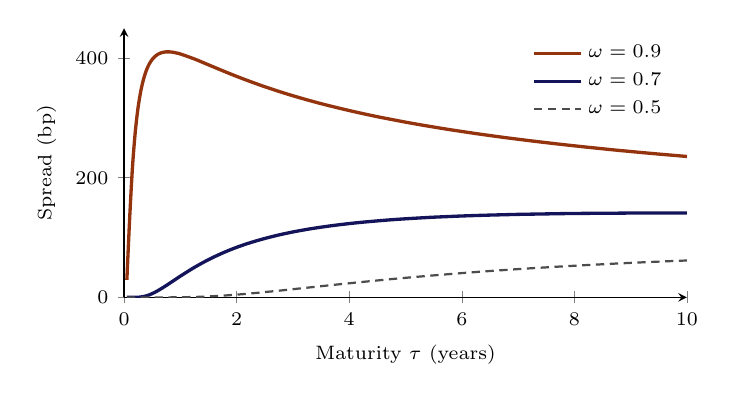
\begin{tikzpicture}[font=\footnotesize]
		\begin{axis}[
				width=0.72\textwidth, height=5.0cm,
				xmin=0, xmax=10, ymin=0, ymax=450,
				xlabel={Maturity $\tau$ (years)}, ylabel={Spread (bp)},
				axis lines=left, axis line style={thin},
				label style={font=\scriptsize}, tick label style={font=\scriptsize},
				legend style={font=\scriptsize, draw=none, fill=none, at={(0.98,0.98)}, anchor=north east},
				legend cell align=left,
			]
			\addplot[RawSienna, very thick, smooth] coordinates {(0.05,29.3) (0.10,132.5) (0.15,218.0) (0.20,277.2) (0.25,317.9) (0.30,346.2) (0.35,366.1) (0.40,380.4) (0.45,390.6) (0.50,397.8) (0.55,402.9) (0.60,406.4) (0.65,408.6) (0.70,409.9) (0.75,410.5) (0.80,410.5) (0.85,410.1) (0.90,409.3) (0.95,408.2) (1.00,407.0) (1.25,398.6) (1.50,388.8) (1.75,379.0) (2.00,369.5) (2.25,360.6) (2.50,352.2) (2.75,344.4) (3.00,337.1) (3.25,330.3) (3.50,323.9) (3.75,318.0) (4.00,312.4) (4.25,307.1) (4.50,302.1) (4.75,297.5) (5.00,293.0) (5.25,288.8) (5.50,284.8) (5.75,281.0) (6.00,277.4) (6.25,273.9) (6.50,270.6) (6.75,267.4) (7.00,264.4) (7.25,261.5) (7.50,258.7) (7.75,256.0) (8.00,253.4) (8.25,250.9) (8.50,248.5) (8.75,246.1) (9.00,243.9) (9.25,241.7) (9.50,239.6) (9.75,237.6) (10.00,235.6)};
			\addlegendentry{$\omega=0.9$}
			\addplot[MidnightBlue!80!black, very thick, smooth] coordinates {(0.05,-0.0) (0.10,0.0) (0.15,0.0) (0.20,0.0) (0.25,0.2) (0.30,0.7) (0.35,1.5) (0.40,2.7) (0.45,4.3) (0.50,6.3) (0.55,8.6) (0.60,11.2) (0.65,14.0) (0.70,16.9) (0.75,19.9) (0.80,23.0) (0.85,26.1) (0.90,29.3) (0.95,32.4) (1.00,35.5) (1.25,50.2) (1.50,63.1) (1.75,74.2) (2.00,83.7) (2.25,91.7) (2.50,98.5) (2.75,104.4) (3.00,109.4) (3.25,113.7) (3.50,117.4) (3.75,120.6) (4.00,123.4) (4.25,125.8) (4.50,127.9) (4.75,129.8) (5.00,131.4) (5.25,132.8) (5.50,134.1) (5.75,135.1) (6.00,136.1) (6.25,136.9) (6.50,137.6) (6.75,138.2) (7.00,138.8) (7.25,139.2) (7.50,139.6) (7.75,140.0) (8.00,140.3) (8.25,140.5) (8.50,140.7) (8.75,140.8) (9.00,141.0) (9.25,141.0) (9.50,141.1) (9.75,141.1) (10.00,141.1)};
			\addlegendentry{$\omega=0.7$}
			\addplot[Gray!60!black, thick, densely dashed, smooth] coordinates {(0.05,-0.0) (0.10,-0.0) (0.15,-0.0) (0.20,0.0) (0.25,0.0) (0.30,0.0) (0.35,0.0) (0.40,0.0) (0.45,0.0) (0.50,0.0) (0.55,0.0) (0.60,0.0) (0.65,0.0) (0.70,0.0) (0.75,0.0) (0.80,0.0) (0.85,0.1) (0.90,0.1) (0.95,0.1) (1.00,0.2) (1.25,0.7) (1.50,1.6) (1.75,2.9) (2.00,4.6) (2.25,6.6) (2.50,8.9) (2.75,11.2) (3.00,13.7) (3.25,16.2) (3.50,18.7) (3.75,21.2) (4.00,23.6) (4.25,26.0) (4.50,28.3) (4.75,30.6) (5.00,32.7) (5.25,34.8) (5.50,36.8) (5.75,38.7) (6.00,40.6) (6.25,42.4) (6.50,44.1) (6.75,45.7) (7.00,47.3) (7.25,48.8) (7.50,50.2) (7.75,51.6) (8.00,52.9) (8.25,54.2) (8.50,55.4) (8.75,56.6) (9.00,57.7) (9.25,58.8) (9.50,59.8) (9.75,60.8) (10.00,61.7)};
			\addlegendentry{$\omega=0.5$}
		\end{axis}
	\end{tikzpicture}
	\caption{The term structure of credit spreads \eqref{eq:merton-spread} with
		$\sigma=20\%$. Low leverage gives a spread rising from zero; high leverage
		gives a hump. (For $\omega\ge1$ the spread explodes as $\tau\to0$: the firm is
		already insolvent in PV terms.)}
	\label{fig:merton-spread}
\end{figure}

\zh{圖：$\sigma=20\%$ 下 credit spread 對期限的曲線。槓桿低時 spread 從 $0$ 開始上升；槓桿高時先升後降。$\omega\ge1$ 時公司以現值計已資不抵債，$\tau\to0$ 時 spread 爆掉。}

\begin{intuition}
	For short maturities a low-leverage firm simply cannot fall far enough in time to default, so the spread starts at zero --- one of the model's well-known weaknesses, since observed short-term spreads are not zero.
	Over long horizons the firm value drifts at $r$ in the risk-neutral world and outruns a debt that does not grow, so the annualized spread eventually declines.
\end{intuition}

\zh{期限很短時，低槓桿的公司來不及跌到違約，所以 spread 從 $0$ 開始——這是模型有名的缺點，因為實際的短期 spread 不是 $0$。期限很長時，risk-neutral 下公司價值以 $r$ 成長、甩開不會成長的負債，所以年化 spread 最後會下降。}

\source{Slide p.~384}

In general, suppose the firm has a dividend yield at rate $q$ and the bankruptcy costs are a constant proportion $\alpha$ of the remaining firm value.
Then \eqref{eq:merton-stock}--\eqref{eq:merton-bond} become, respectively,\footnote{Collin-Dufresne \& Goldstein (2000).}
\begin{align*}
	nS & \;=\; Ve^{-q\tau}N(x)-Xe^{-r\tau}N\bigl(x-\sigma\sqrt{\tau}\bigr) ,                \\
	B  & \;=\; (1-\alpha)\,Ve^{-q\tau}N(-x)+Xe^{-r\tau}N\bigl(x-\sigma\sqrt{\tau}\bigr) ,
\end{align*}
with $x\triangleq\bigl[\ln(V/X)+(r-q+\sigma^{2}/2)\tau\bigr]/(\sigma\sqrt{\tau})$ as in \eqref{eq:bs-x-q}.
The stock is unaffected by bankruptcy costs --- it gets nothing in default anyway --- while the bondholders recover only $(1-\alpha)V^{*}$.

\zh{一般情況：公司有 dividend yield $q$、破產成本是剩餘價值的固定比例 $\alpha$，股票和債券就變成上面兩式。股票不受破產成本影響（違約時本來就拿不到），債權人則只拿回 $(1-\alpha)V^{*}$。}

\begin{remark}[補充]
	\textbf{$B$ 怎麼來。}到期時債券的 payoff 是 $(1-\alpha)V^{*}\mathbf{1}_{\{V^{*}\le X\}}+X\mathbf{1}_{\{V^{*}>X\}}$，分兩項取現值：
	\begin{enumerate}[(1),nosep]
		\item call 的公式 $Ve^{-q\tau}N(x)-Xe^{-r\tau}N(x-\sigma\sqrt{\tau})$ 中，第一項是 $V^{*}\mathbf{1}_{\{V^{*}>X\}}$ 的現值、第二項是 $X\mathbf{1}_{\{V^{*}>X\}}$ 的現值。
		\item $V^{*}$ 本身的現值是 $Ve^{-q\tau}$（\autoref{sec:continuous-yield}），所以 $V^{*}\mathbf{1}_{\{V^{*}\le X\}}$ 的現值是 $Ve^{-q\tau}\bigl(1-N(x)\bigr)=Ve^{-q\tau}N(-x)$，乘上 $(1-\alpha)$。
		\item 兩項相加就是上面的 $B$。$\alpha=0$、$q=0$ 時回到 \eqref{eq:merton-bond}。
	\end{enumerate}
\end{remark}

\subsection{A Numerical Example}
\label{sec:merck-example}

\source{Slides pp.~385--388}

XYZ.com's assets consist of 1,000 shares of Merck as of March 20, 1995, when Merck's market value per share is \$44.5.
It issues 1,000 shares of XYZ.com common stock and 30 zero-coupon bonds maturing on July 21, 1995, each promising to pay \$1,000 at maturity.
So
\[
	n=1{,}000 , \qquad V=44.5\times n=44{,}500 , \qquad X=30\times1{,}000=30{,}000 .
\]
As the Merck calls are being traded, we do not need formulas to price them (\autoref{tab:merck}).

\zh{XYZ.com 的資產是 1995/3/20 的 1000 股 Merck（每股 44.5），發行 1000 股普通股和 30 張 1995/7/21 到期、各付 1000 的 zero-coupon bond：$n=1000$、$V=44{,}500$、$X=30{,}000$。Merck 的 call 有在交易，所以直接用報價，不需要公式。}

\begin{table}[H]
	\centering
	\small
	\begin{tabular}{lllrrrr}
		\toprule
		         &        &      & \multicolumn{2}{c}{Call} & \multicolumn{2}{c}{Put}                                   \\
		\cmidrule(lr){4-5}\cmidrule(lr){6-7}
		Option   & Strike & Exp. & Vol.                     & Last                    & Vol.  & Last                     \\
		\midrule
		Merck    & 30     & Jul  & 328                      & $15\frac14$             & \ldots & \ldots                  \\
		$44\frac12$ & 35  & Jul  & 150                      & $9\frac12$              & 10    & $\frac1{16}$             \\
		$44\frac12$ & 40  & Apr  & 887                      & $4\frac34$              & 136   & $\frac1{16}$             \\
		$44\frac12$ & 40  & Jul  & 220                      & $5\frac12$              & 297   & $\frac14$                \\
		$44\frac12$ & 40  & Oct  & 58                       & $6$                     & 10    & $\frac12$                \\
		$44\frac12$ & 45  & Apr  & 3050                     & $\frac78$               & 100   & $1\frac18$               \\
		$44\frac12$ & 45  & May  & 462                      & $1\frac38$              & 50    & $1\frac38$               \\
		$44\frac12$ & 45  & Jul  & 883                      & $1\frac{15}{16}$        & 147   & $1\frac34$               \\
		$44\frac12$ & 45  & Oct  & 367                      & $2\frac34$              & 188   & $2\frac1{16}$            \\
		\bottomrule
	\end{tabular}
	\caption{Merck option quotations, March 20, 1995 (textbook Fig.~11.1).}
	\label{tab:merck}
\end{table}

The Merck option relevant for pricing is the July call with a strike price of $X/n=30$ dollars, selling for \$15.25.
So XYZ.com's stock is worth $15.25\times n=15{,}250$ dollars, and the entire bond issue is worth
\[
	B \;=\; 44{,}500-15{,}250 \;=\; 29{,}250
\]
dollars, or \$975 per bond.

\zh{要用的是 strike $X/n=30$ 的 July call，價格 15.25，所以股票值 $15{,}250$，債券總值 $44{,}500-15{,}250=29{,}250$，每張 975。}

The XYZ.com bonds are equivalent to a default-free zero-coupon bond with \$$X$ par value plus $n$ written European puts on Merck at a strike price of \$30, by put--call parity (\autoref{thm:put-call-parity}).

\begin{remark}
	\begin{enumerate}[(1),nosep]
		\item \textbf{為什麼用 strike $X/n$ 的 Merck call。}記 $M^{*}$ 為到期時一股 Merck 的價格，$V^{*}=nM^{*}$。股票的 payoff 是 $\max(V^{*}-X,0)=n\max(M^{*}-X/n,0)$，也就是 $n$ 個 strike $X/n=30$ 的 Merck call。
		\item \textbf{債券 $=$ riskless bond $-$ puts。}由 parity，$B=V-C=Xe^{-r\tau}-P$，$P$ 是標的 $V$、strike $X$ 的 put；同 (1)，$P$ 就是 $n$ 個 strike $30$ 的 Merck put。
	\end{enumerate}
\end{remark}
The difference between $B$ and the price of the default-free bond is the value of these puts.

\zh{由 put--call parity，XYZ.com 的債券等於面額 $X$ 的無違約 zero-coupon bond 加上賣出 $n$ 個 strike 30 的 Merck European put；$B$ 和無違約債券價格的差就是這些 put 的價值。}

\source{Slides pp.~389--390}

\autoref{tab:capital-structure} shows the total market values of the XYZ.com stock and bonds under various debt amounts $X$.
For example, if the promised payment is \$45,000, the relevant option is the July call with a strike price of $45{,}000/n=45$ dollars; since it sells for $\$1\frac{15}{16}$, the stock is worth $(1+15/16)\times n=1{,}937.5$ dollars.

\begin{table}[H]
	\centering
	\begin{tabular}{rrrr}
		\toprule
		Promised payment & Current market & Current market & Current total \\
		to bondholders   & value of bonds & value of stock & value of firm \\
		$X$              & $B$            & $nS$           & $V$           \\
		\midrule
		30{,}000         & 29{,}250.0     & 15{,}250.0     & 44{,}500      \\
		35{,}000         & 35{,}000.0     & 9{,}500.0      & 44{,}500      \\
		40{,}000         & 39{,}000.0     & 5{,}500.0      & 44{,}500      \\
		45{,}000         & 42{,}562.5     & 1{,}937.5      & 44{,}500      \\
		\bottomrule
	\end{tabular}
	\caption{Distribution of corporate value under alternative capital
		structures, from the July calls in \autoref{tab:merck}. The last column
		never changes.}
	\label{tab:capital-structure}
\end{table}

The market value of the stock decreases as the debt-to-equity ratio increases.

\zh{\autoref{tab:capital-structure} 列出不同負債 $X$ 下股票和債券的市值；例如承諾支付 45{,}000 時用 strike 45 的 July call（$1\frac{15}{16}$），股票值 1{,}937.5。負債比例越高股票越不值錢；公司總價值那一欄不變。}

\begin{remark}
	\autoref{tab:capital-structure} 每一列都用同一個方法：$nS=n\times(\text{strike }X/n\text{ 的 July call 價格})$，$B=V-nS$，$V=44{,}500$ 固定。
\end{remark}

\begin{note}
	$X=35{,}000$ 那一列看起來很怪：$B=35{,}000$ 表示債券以 par 出售，也就是四個月的 yield 為\emph{零}。
	這只是報價造成的：July 35 call 最後成交價是 $9\frac12$，剛好等於 intrinsic value $44.5-35$，所以隱含的 put 價值為零，利息也被忽略了。
	1995 年那些過時或四捨五入的報價，本來就不會精確到每一分錢都符合 no-arbitrage。
\end{note}

\subsection{Conflicts between Stockholders and Bondholders}
\label{sec:claim-dilution}

\source{Slides pp.~391--395}

There are conflicts between stockholders and bondholders.
An option's terms cannot be changed after issuance, but a firm can change its capital structure.
There lies one key difference between options and corporate securities: parameters such as volatility,\footnote{This is called the \vocab{asset substitution problem} (Myers, 1977).} dividend, and strike price are under partial control of the stockholders or boards.

\zh{股東和債權人之間有利益衝突。option 發行後條款不能改，公司卻可以改資本結構——這是 option 和公司證券的關鍵差別：volatility（asset substitution problem）、股利、strike 等參數部分由股東或董事會控制。}

\paragraph{Issuing more debt.}
Suppose XYZ.com issues 15 more bonds with the same terms to buy back stock.
The total debt is now $X=45{,}000$ dollars, and \autoref{tab:capital-structure} says the total market value of the bonds should be \$42,562.5.
The new bondholders pay
\[
	42{,}562.5\times(15/45) \;=\; 14{,}187.5
\]
dollars, and the remaining stock is worth \$1,937.5.
The stockholders therefore gain
\[
	14{,}187.5+1{,}937.5-15{,}250 \;=\; 875
\]
dollars, and the original bondholders lose an equal amount,
\[
	29{,}250-\frac{30}{45}\times42{,}562.5 \;=\; 875 .
\]
This is called \vocab{claim dilution}.\footnote{Fama \& M.~H.~Miller (1972).}

\zh{發新債：再發 15 張同條件債券買回股票，總負債 45{,}000，由表所有債券值 42{,}562.5。新債權人付 $42{,}562.5\times15/45=14{,}187.5$，剩下股票值 1{,}937.5；股東賺 875，原債權人賠 875，這叫 claim dilution。}

\begin{remark}
	\textbf{數字從哪來。}
	\begin{enumerate}[(1),nosep]
		\item 發新債後總面額 $45{,}000$，由 \autoref{tab:capital-structure}，所有債券合起來值 $42{,}562.5$。新舊債券條件相同，依面額分：新的 $15$ 張占 $15/45$，舊的 $30$ 張占 $30/45$。
		\item \textbf{股東。}原本有 $15{,}250$ 的股票；之後拿到新債的錢 $14{,}187.5$（拿去買回股票，錢回到股東手上），加上剩下的股票 $1{,}937.5$。差額 $875$。
		\item \textbf{原債權人。}原本 $29{,}250$，之後只值 $\frac{30}{45}\times42{,}562.5=28{,}375$，少了 $875$。
	\end{enumerate}
	$V$ 不變，所以股東賺的就是原債權人賠的。
\end{remark}

\begin{remark}
	\vocab{債權稀釋}（claim dilution）：新發行同等順位的債券，讓原債權人在違約時要和更多人分 $V^{*}$，違約機率也變高。股東拿新債的錢買回股票，等於把原債權人的一部分價值移轉給自己；公司總價值 $V$ 不變，只是分配變了。
\end{remark}

\paragraph{Paying a dividend.}
Suppose instead the stockholders sell $(1/3)\times n$ Merck shares to fund a \$14,833.3 cash dividend.
The stockholders now have \$14,833.3 in cash plus a call on $(2/3)\times n$ Merck shares, and the strike price remains $X=30{,}000$.
This is equivalent to owning $2/3$ of a call on $n$ Merck shares with a strike price of \$45,000, since $\max\bigl(\tfrac23V^{*}-30{,}000,0\bigr)=\tfrac23\max(V^{*}-45{,}000,0)$.
As $n$ such calls are worth \$1,937.5 (\autoref{tab:capital-structure}), the XYZ.com stock is worth $(2/3)\times1{,}937.5=1{,}291.67$ dollars, and the bonds are worth
\[
	(2/3)\times n\times44.5-1{,}291.67 \;=\; 28{,}375
\]
dollars.
Hence the stockholders gain $14{,}833.3+1{,}291.67-15{,}250\approx875$ dollars, and the bondholders watch their value drop from \$29,250 to \$28,375, a loss of \$875.

\zh{發股利：改為賣掉 $\frac13n$ 股 Merck 發 14{,}833.3 現金股利。股東有現金加上 $\frac23n$ 股 Merck 上 strike 30{,}000 的 call，等於 $\frac23$ 個 strike 45{,}000 的 call，值 1{,}291.67；債券值 28{,}375。股東同樣賺約 875、債權人賠 875。}

\begin{remark}
	\begin{enumerate}[(1),nosep]
		\item \textbf{股利金額。}賣掉 $\frac13n$ 股 Merck，每股 $44.5$：$\frac13\times1{,}000\times44.5=14{,}833.3$。
		\item \textbf{等價的 call。}公司剩下 $\frac23n$ 股 Merck，到期價值 $\frac23V^{*}$，債務仍是 $30{,}000=\frac23\times45{,}000$，所以股票 payoff 是 $\max\bigl(\frac23V^{*}-\frac23\times45{,}000,0\bigr)=\frac23\max(V^{*}-45{,}000,0)$。
		\item \textbf{債券。}公司現在的總價值是 $\frac23\times44{,}500$，扣掉股票 $1{,}291.67$ 就是債券 $28{,}375$。
	\end{enumerate}
\end{remark}

\begin{moral}
	Two different actions, the same \$875 transfer --- because both leave the bondholders with the same claim: $2/3$ of the old firm against the old promise.
	The same logic explains why bondholders loathe risky investments: the stock is a call, its vega is positive (\autoref{sec:vega}), and raising $\sigma$ moves value from the bonds to the stock with $V$ unchanged.
	Covenants in bond indentures exist to limit exactly these moves.
\end{moral}

\zh{兩種做法轉移的都是 875，因為債權人最後面對同樣的處境：只剩原公司的 $\frac23$，承諾的金額卻不變。同理，債權人討厭高風險投資：股票是 call、vega 為正，提高 $\sigma$ 會在 $V$ 不變下把價值從債券移到股票。債券契約的 covenants 就是要限制這些動作。}

\subsection{Further Topics}
\label{sec:corporate-further}

\source{Slides pp.~396--397}

Other examples:\footnote{Cox \& Rubinstein (1985); Geske (1977). See Section 11.1 of the textbook.}
\begin{itemize}[itemsep=0.3em]
	\item \textbf{Stock as a compound call} when the company issues coupon bonds: paying each coupon buys the right to keep the firm until the next payment --- an option on an option.
	\item \textbf{Subordinated debts as bull call spreads.} With senior debt $X_{s}$ and junior debt $X_{j}$ of the same maturity, the junior debt pays $0$, $V^{*}-X_{s}$, or $X_{j}$ according as $V^{*}\le X_{s}$, $X_{s}<V^{*}\le X_{s}+X_{j}$, or $V^{*}>X_{s}+X_{j}$: a long $X_{s}$ call and a short $X_{s}+X_{j}$ call on $V$ (\autoref{sec:bull-spreads}).

	\textit{說明：}senior 先拿，junior 拿剩下的、最多 $X_{j}$，所以 junior 的 payoff 是 $\min\bigl(\max(V^{*}-X_{s},0),\,X_{j}\bigr)=\max(V^{*}-X_{s},0)-\max(V^{*}-X_{s}-X_{j},0)$；逐段檢查三種情況即可驗證。
	\item \textbf{Warrants as calls.} A warrant is a call issued by the firm on its own new shares. With $n$ shares and $m$ warrants of strike $X$, each warrant is worth $W=\frac{n}{n+m}\,C$, where $C$ is the call value on $S+(m/n)W$; the dilution makes this an equation in $W$ to solve numerically.

	\textit{說明：}warrant 被履約時，公司收到 $mX$ 並發行 $m$ 股新股。記到期時公司的總價值（股票 $+$ warrant）為 $V^{*}$，履約後公司值 $V^{*}+mX$，由 $n+m$ 股平分，所以每個 warrant 的 payoff 是
	\[
		\frac{V^{*}+mX}{n+m}-X=\frac{n}{n+m}\Bigl(\frac{V^{*}}{n}-X\Bigr) .
	\]
	也就是 $\frac{n}{n+m}$ 個標的為 $V/n$、strike 為 $X$ 的 call。今天 $V=nS+mW$，所以 $V/n=S+(m/n)W$；$W$ 同時出現在兩邊，要用數值方法解。
	\item \textbf{Callable bonds as American calls with 2 strike prices.} If the firm may call the bonds at any time for $X_{c}$, the stock is an American call on $V$ with strike $X_{c}$ before maturity and $X$ at maturity.
	\item \textbf{Convertible bonds}: bonds the holder may convert into new shares, adding a call on a fraction of the firm.
	\item \textbf{Bonds with safety covenants as barrier options}: if the firm must pass to the bondholders when $V$ falls below $H$, the stock is a down-and-out call (\autoref{sec:barrier}).
\end{itemize}
Securities issued by firms with a complex capital structure must be solved by numerical methods such as trees.\footnote{T.~Dai (\texttt{B82506025}, \texttt{R86526008}, \texttt{D8852600}), Lyuu, \& C.~Wang (\texttt{F95922018}) (2010).}

\zh{其他例子：發 coupon bond 時股票是 compound call（每付一次 coupon 就買到繼續持有公司到下次付款的權利）；次順位債是 bull call spread；warrant 是 call；可贖回債券讓股票成為有兩個 strike 的 American call；可轉債加上一個對部分公司的 call；有安全條款的債券讓股票成為 down-and-out call。資本結構複雜時只能用 tree 等數值方法。}

\subsection{Distance to Default}

\source{Slide p.~398}

Let $\mu$ be the total value $V$'s rate of expected return.\footnote{This parameter is generally hard to estimate. Campbell, Hilscher, and Szilagyi (2008) use $r+0.06$ for simplicity.}
The firm defaults at maturity exactly when $V^{*}<X$.
Under the real-world dynamics, $\ln(V^{*}/V)\sim N\bigl((\mu-\sigma^{2}/2)\tau,\ \sigma^{2}\tau\bigr)$ (\autoref{sec:toward-bs} with $\mu-\sigma^{2}/2$ for the log drift), so by \autoref{prop:lognormal-tail} the probability of default $\tau$ years from now equals
\[
	N(-\mathrm{DTD}) ,
	\qquad\text{where}\qquad
	\mathrm{DTD} \;\triangleq\; \frac{\ln(V/X)+(\mu-\sigma^{2}/2)\,\tau}{\sigma\sqrt{\tau}} .
\]
$V/X$ is called the \vocab{leverage ratio}.\footnote{Merton (1974). Useful in forecasting defaults (Bharath \& Shumway, 2008).}

\zh{令 $\mu$ 為公司價值 $V$ 的期望報酬率。到期違約恰好是 $V^{*}<X$；真實世界下 $\ln(V^{*}/V)\sim N((\mu-\sigma^{2}/2)\tau,\sigma^{2}\tau)$，所以 $\tau$ 年後違約機率是 $N(-\mathrm{DTD})$。$V/X$ 叫 leverage ratio。}

\begin{remark}
	\vocab{違約距離}（distance to default, DTD）。
	\begin{enumerate}[(1),nosep]
		\item \textbf{違約機率的推導。}$\ln V^{*}\sim N(m,s^{2})$，$m=\ln V+(\mu-\sigma^{2}/2)\tau$、$s=\sigma\sqrt{\tau}$。由 \autoref{prop:lognormal-tail}，$\mathrm{Prob}[V^{*}>X]=N\bigl(\frac{m-\ln X}{s}\bigr)=N(\mathrm{DTD})$，所以 $\mathrm{Prob}[V^{*}<X]=1-N(\mathrm{DTD})=N(-\mathrm{DTD})$。
		\item \textbf{DTD 的意思。}$\mathrm{DTD}=\frac{m-\ln X}{s}$：$\ln V^{*}$ 的平均 $m$ 離違約門檻 $\ln X$ 有幾個標準差 $s$。DTD 越大越安全。
		\item \textbf{和 \eqref{eq:merton-stock} 的關係。}$N(x-\sigma\sqrt{\tau})$ 是 risk-neutral 下不違約的機率；DTD 只是把其中的 $r$ 換成真實的 $\mu$。
	\end{enumerate}
\end{remark}

%─────§ Barrier options──────────────────────────────────────────────────────────────────────────────────────────────────────────────────────────────
\section{Barrier Options}
\label{sec:barrier}

\source{Slides pp.~399--401}

\vocab{Barrier options} have a payoff that depends on whether the underlying asset's price reaches a certain price level $H$ throughout its life.\footnote{A former MBA student in finance told the lecturer on March 26, 2004, that she did not understand why barrier options were covered until she started working in a bank. She was working for Lehman Brothers in Hong Kong as of April, 2006.}

\zh{barrier option 的 payoff 取決於標的價格在存續期間有沒有碰到某個水準 $H$。}

\begin{definition}
	\begin{itemize}[nosep]
		\item A \vocab{knock-out} (KO) option is an ordinary European option which ceases to exist if the barrier $H$ is reached by the price of its underlying asset.
		      A knock-out call is sometimes called a \vocab{down-and-out} option if $H<S$; a knock-out put is sometimes called an \vocab{up-and-out} option when $H>S$.
		\item A \vocab{knock-in} (KI) option comes into existence if a certain barrier is reached.
		      A \vocab{down-and-in} option is a knock-in call that comes into existence only when the barrier is reached and $H<S$; an \vocab{up-and-in} option is a knock-in put that comes into existence only when the barrier is reached and $H>S$.
	\end{itemize}
\end{definition}

\zh{knock-out（KO）：一般的 European option，標的一碰到 $H$ 就作廢；$H<S$ 的 knock-out call 叫 down-and-out，$H>S$ 的 knock-out put 叫 up-and-out。knock-in（KI）：碰到 $H$ 才生效；$H<S$ 的叫 down-and-in call，$H>S$ 的叫 up-and-in put。}

\begin{remark}
	\vocab{障礙選擇權}（barrier option）：報酬取決於存續期間內股價是否\emph{碰過}障礙 $H$。\vocab{出局}（knock-out）型一碰就作廢；\vocab{入局}（knock-in）型要碰到才生效。down/up 指障礙在目前股價的下方或上方。
\end{remark}

\begin{figure}[H]
	\centering
	\begin{tikzpicture}[font=\small, >={Stealth[length=5pt]}]
		\draw[->] (0,0) -- (7.2,0) node[right] {Time};
		\draw[->] (0,0) -- (0,4.0) node[above] {Price};
		\draw[Gray!70!black] (0,2.7) node[left, text=black] {$H$} -- (6.8,2.7);
		\node[left] at (0,1.3) {$S$};
		\draw[MidnightBlue!80!black, thick, densely dotted]
		(0,1.3) .. controls (0.8,1.1) and (1.2,1.9) .. (1.8,1.7)
		.. controls (2.3,1.5) and (2.6,2.2) .. (3.0,2.7)
		.. controls (3.4,3.25) and (4.1,3.3) .. (4.6,2.6)
		.. controls (5.2,1.8) and (5.9,1.5) .. (6.8,1.6);
		\draw[<-, thick] (3.02,2.62) -- (3.9,1.6) node[below right=-2pt] {barrier hit};
	\end{tikzpicture}
	\caption{A price path that touches the barrier $H$: a knock-out option on this
		path is dead from that moment on, and a knock-in option comes alive --- even
		though the path ends below $H$.}
	\label{fig:barrier-path}
\end{figure}

\zh{圖：一條碰到 $H$ 的路徑：knock-out option 從那一刻起作廢，knock-in option 則生效——即使最後停在 $H$ 下方。}

The two kinds are tied by a parity relation.

\begin{proposition}[In--out parity]
	\label{prop:in-out-parity}
	A European call is equivalent to a portfolio of a European down-and-out call and a European down-and-in call with an identical barrier and strike.
	Likewise for puts with up-and-out and up-and-in.
\end{proposition}

\begin{proof}
	On every path exactly one of the two barrier options is alive at expiration, and the live one pays $\max(S_{\tau}-X,0)$.
	So the portfolio's payoff equals the call's path by path; apply \autoref{cor:same-payoff}.
\end{proof}

The argument never used that $H$ is constant, so the parity holds for any barrier.\footnote{Comment 11.2.1 of the textbook.}
Formulas exist for all the possible barrier options mentioned above.\footnote{Haug (2006).}

\zh{兩種 barrier option 由 in--out parity 連起來：同 barrier、同 strike 的 down-and-out call 加 down-and-in call 等於普通 European call（put 的 up-and-out 加 up-and-in 同理），因為每條路徑上恰好一個活著，活著的付 $\max(S_{\tau}-X,0)$。證明沒用到 $H$ 是常數，所以任何 barrier 都成立。上面所有 barrier option 都有公式。}

\subsection{Merton's Formulas}

\source{Slides pp.~402--403}

\begin{theorem}[Merton, 1973]
	\label{thm:down-and-in}
	Assume $X\ge H$.
	The value of a European down-and-in call on a stock paying a dividend yield of $q$ is
	\begin{equation}
		Se^{-q\tau}\Bigl(\frac{H}{S}\Bigr)^{2\lambda}N(x)-Xe^{-r\tau}\Bigl(\frac{H}{S}\Bigr)^{2\lambda-2}N\bigl(x-\sigma\sqrt{\tau}\bigr) ,
		\label{eq:down-and-in}
	\end{equation}
	where
	\[
		x \;\triangleq\; \frac{\ln\bigl(H^{2}/(SX)\bigr)+\bigl(r-q+\sigma^{2}/2\bigr)\tau}{\sigma\sqrt{\tau}} ,
		\qquad
		\lambda \;\triangleq\; \frac{r-q+\sigma^{2}/2}{\sigma^{2}} .
	\]
\end{theorem}

See Exercise 17.1.6 of the textbook for a proof.
A European down-and-out call can then be priced via the in--out parity: \eqref{eq:bs-call-q} minus \eqref{eq:down-and-in}.

\zh{Merton 的公式（$X\ge H$）：有 dividend yield $q$ 的 European down-and-in call 值 \eqref{eq:down-and-in}，證明見課本 Exercise 17.1.6。down-and-out call 由 in--out parity 得到：\eqref{eq:bs-call-q} 減 \eqref{eq:down-and-in}。}

\begin{theorem}[Merton, 1973]
	Assume $X\le H$.
	The value of a European up-and-in put is
	\[
		Xe^{-r\tau}\Bigl(\frac{H}{S}\Bigr)^{2\lambda-2}N\bigl(-x+\sigma\sqrt{\tau}\bigr)-Se^{-q\tau}\Bigl(\frac{H}{S}\Bigr)^{2\lambda}N(-x) .
	\]
\end{theorem}

Again, a European up-and-out put can be priced via the in--out parity.

\zh{$X\le H$ 時 up-and-in put 也有類似公式；up-and-out put 一樣用 in--out parity。}

\begin{figure}[H]
	\centering
	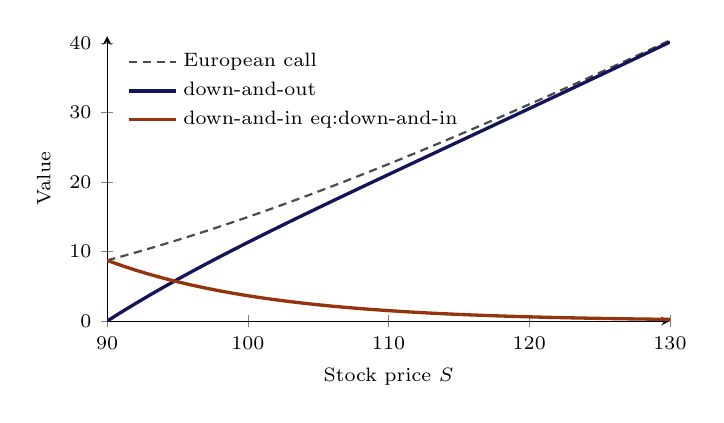
\begin{tikzpicture}[font=\footnotesize]
		\begin{axis}[
				width=0.72\textwidth, height=5.2cm,
				xmin=90, xmax=130, ymin=0, ymax=41,
				xlabel={Stock price $S$}, ylabel={Value},
				axis lines=left, axis line style={thin},
				label style={font=\scriptsize}, tick label style={font=\scriptsize},
				legend style={font=\scriptsize, draw=none, fill=none, at={(0.02,0.98)}, anchor=north west},
				legend cell align=left,
			]
			\addplot[Gray!60!black, thick, densely dashed] coordinates {(90,8.7371) (91,9.2871) (92,9.8545) (93,10.4389) (94,11.0399) (95,11.6574) (96,12.2907) (97,12.9397) (98,13.6038) (99,14.2826) (100,14.9758) (101,15.6829) (102,16.4034) (103,17.1370) (104,17.8832) (105,18.6416) (106,19.4116) (107,20.1930) (108,20.9853) (109,21.7880) (110,22.6007) (111,23.4230) (112,24.2546) (113,25.0950) (114,25.9438) (115,26.8007) (116,27.6653) (117,28.5373) (118,29.4163) (119,30.3020) (120,31.1941) (121,32.0922) (122,32.9960) (123,33.9054) (124,34.8199) (125,35.7394) (126,36.6635) (127,37.5921) (128,38.5248) (129,39.4616) (130,40.4021)};
			\addlegendentry{European call}
			\addplot[MidnightBlue!80!black, very thick] coordinates {(90,0.0000) (91,1.2738) (92,2.5063) (93,3.7017) (94,4.8640) (95,5.9968) (96,7.1035) (97,8.1868) (98,9.2497) (99,10.2945) (100,11.3234) (101,12.3384) (102,13.3414) (103,14.3340) (104,15.3176) (105,16.2936) (106,17.2631) (107,18.2272) (108,19.1869) (109,20.1430) (110,21.0961) (111,22.0471) (112,22.9964) (113,23.9446) (114,24.8921) (115,25.8393) (116,26.7866) (117,27.7342) (118,28.6823) (119,29.6313) (120,30.5812) (121,31.5322) (122,32.4844) (123,33.4380) (124,34.3929) (125,35.3493) (126,36.3072) (127,37.2667) (128,38.2276) (129,39.1902) (130,40.1542)};
			\addlegendentry{down-and-out}
			\addplot[RawSienna, very thick] coordinates {(90,8.7371) (91,8.0133) (92,7.3482) (93,6.7372) (94,6.1759) (95,5.6605) (96,5.1873) (97,4.7528) (98,4.3541) (99,3.9881) (100,3.6524) (101,3.3445) (102,3.0620) (103,2.8031) (104,2.5656) (105,2.3480) (106,2.1485) (107,1.9658) (108,1.7984) (109,1.6450) (110,1.5045) (111,1.3759) (112,1.2581) (113,1.1503) (114,1.0517) (115,0.9614) (116,0.8787) (117,0.8032) (118,0.7340) (119,0.6707) (120,0.6129) (121,0.5600) (122,0.5116) (123,0.4674) (124,0.4270) (125,0.3900) (126,0.3563) (127,0.3254) (128,0.2972) (129,0.2714) (130,0.2479)};
			\addlegendentry{down-and-in \eqref{eq:down-and-in}}
		\end{axis}
	\end{tikzpicture}
	\caption{Down-and-in and down-and-out calls with $X=100$, $H=90$, $r=10\%$,
		$\sigma=25\%$, $\tau=1$, $q=0$, as functions of $S\ge H$. At $S=H$ the
		down-and-in call \emph{is} the European call and the down-and-out call is
		worthless; the two always add up to the European call. At $S=95$ the
		down-and-in call is worth $5.6605$.}
	\label{fig:down-and-in}
\end{figure}

\zh{圖：$X=100$、$H=90$、$r=10\%$、$\sigma=25\%$、$\tau=1$、$q=0$ 的 down-and-in 和 down-and-out call 對 $S\ge H$ 作圖。$S=H$ 時 down-and-in 就是普通 call、down-and-out 為 $0$；兩者相加永遠是普通 call。$S=95$ 時 down-and-in 值 5.6605。}

\begin{note}
	兩個 sanity check。
	當 $S=H$ 時，$(H/S)^{\cdot}=1$，且 $\frac{H^{2}}{SX}=\frac{H}{X}=\frac{S}{X}$，所以 $x$ 變成 \eqref{eq:bs-x-q}，\eqref{eq:down-and-in} 化簡為 \eqref{eq:bs-call-q}：barrier 一開始就被碰到，down-and-in call 就是普通的 call。
	當 $S\to\infty$ 時，因子 $(H/S)^{2\lambda}$ 讓價值趨近零：barrier 太遠，碰不到。
\end{note}

\subsection{Popularity}

\source{Slide p.~404}

Knock-out options were issued in the U.S.\ in 1967.\footnote{Cox \& Rubinstein (1985).}
Knock-in puts are the most popular barrier options, knock-out puts are the second most popular, and knock-out calls are the most popular among barrier call options.\footnote{Bennett (2014).}

\zh{knock-out option 1967 年在美國發行。knock-in put 最受歡迎、knock-out put 第二；call 之中最受歡迎的是 knock-out call。}

\begin{intuition}
	Barrier options are cheaper than their vanilla counterparts (by in--out parity each piece is worth less than the whole), and the buyer gives up only scenarios they consider unlikely or irrelevant.
	A knock-in put, for instance, is crash insurance that only switches on once the market has already fallen through $H$.
\end{intuition}

\zh{barrier option 比普通 option 便宜（由 in--out parity，每一部分都小於整體），買方只放棄自己認為不太可能或不重要的情境。例如 knock-in put 是市場跌破 $H$ 後才啟動的崩盤保險。}

\subsection{Are American Options Barrier Options?}
\label{sec:american-vs-barrier}

\source{Slides pp.~405--406}

American options look like barrier options with the exercise boundary (\autoref{sec:exercise-boundary}) as the barrier and the payoff as the rebate.\footnote{Contributed by Mr.~Yang, Jui-Chung (\texttt{D97723002}) on March 25, 2009.}
One salient difference is that the exercise boundary must be found by backward induction; it cannot be specified arbitrarily.
But the barrier is fixed by a contract,\footnote{Cox \& Rubinstein (1985).} and the barrier option remains European-style, without the right to early exercise.\footnote{Contributed by Ms.~Chen, Sin-Huei (Amber) (\texttt{P00922005}) on March 31, 2021.}

\zh{American option 看起來像 barrier option：barrier 是 exercise boundary、rebate 是 payoff。差別在於 exercise boundary 要由 backward induction 求出，不能任意指定；barrier 則由合約固定，而且 barrier option 仍是 European 式，不能提前履約。}

They become equal if the barrier happens to be identical to the exercise boundary and the rebate equals the intrinsic value.\footnote{Contributed by Mr.~Chuang, Chin-Yu (\texttt{D12922014}) and Mr.~Hsiao, Huan-Wen (\texttt{B90902081}, \texttt{R94922010}, \texttt{D13922016}) on October 2, 2025.}
One can also have American barrier options; one then needs to specify whether the option can be exercised early if the stock price has not touched the barrier.\footnote{Contributed by Mr.~Lu, Yu-Ming (\texttt{R06723032}, \texttt{D08922008}) on March 31, 2021.}

\zh{若 barrier 恰好等於 exercise boundary、rebate 等於 intrinsic value，兩者就相同。也有 American barrier option，這時要規定還沒碰到 barrier 時能不能提前履約。}

\subsection{Interesting Observations}
\label{sec:barrier-reflection}

\source{Slides pp.~407--408}

Assume $H<X$ and write $C(S)$ for the Merton formula \eqref{eq:bs-call-q} as a function of the stock price.
\begin{itemize}[itemsep=0.3em]
	\item Replace $S$ in \eqref{eq:bs-call-q} with $H^{2}/S$.
	      Then \eqref{eq:down-and-in} becomes $C(H^{2}/S)$ when $r-q=\sigma^{2}/2$, and $(S/H)\,C(H^{2}/S)$ when $r-q=0$.
	\item Conversely, replace $S$ in \eqref{eq:down-and-in} with $H^{2}/S$.
	      It becomes $C(S)$ when $r-q=\sigma^{2}/2$, and $(H/S)\,C(S)$ when $r-q=0$.\footnote{Contributed by Mr.~Chou, Ming-Hsin (\texttt{R02723073}) on April 24, 2014.}
\end{itemize}

\zh{設 $H<X$，$C(S)$ 為 \eqref{eq:bs-call-q}。(1) 把 $S$ 換成 $H^{2}/S$：$r-q=\sigma^{2}/2$ 時 \eqref{eq:down-and-in} 等於 $C(H^{2}/S)$，$r=q$ 時等於 $\frac SH C(H^{2}/S)$。(2) 反過來把 \eqref{eq:down-and-in} 的 $S$ 換成 $H^{2}/S$，分別變成 $C(S)$ 和 $\frac HS C(S)$。}

\begin{proof}[Verification（補充；簡報只給結論）]
	記 \eqref{eq:down-and-in} 為 $\mathrm{DI}(S)$。
	\begin{enumerate}[(1),nosep]
		\item \textbf{$r-q=\sigma^{2}/2$。}$\lambda=\frac{\sigma^{2}/2+\sigma^{2}/2}{\sigma^{2}}=1$，所以 $(H/S)^{2\lambda}=(H/S)^{2}$、$(H/S)^{2\lambda-2}=1$：
		\[
			\mathrm{DI}(S)=\frac{H^{2}}{S}e^{-q\tau}N(x)-Xe^{-r\tau}N(x-\sigma\sqrt{\tau}) .
		\]
		$x$ 的分子 $\ln\frac{H^{2}}{SX}=\ln\frac{H^{2}/S}{X}$，正是 \eqref{eq:bs-x-q} 把 $S$ 換成 $H^{2}/S$。所以 $\mathrm{DI}(S)=C(H^{2}/S)$。
		\item \textbf{$r=q$。}$\lambda=\frac12$，$(H/S)^{2\lambda}=\frac HS$、$(H/S)^{2\lambda-2}=\frac SH$：
		\[
			\begin{aligned}
				\mathrm{DI}(S) & =He^{-q\tau}N(x)-\frac{S}{H}Xe^{-r\tau}N(x-\sigma\sqrt{\tau})                                       \\
				               & =\frac{S}{H}\Bigl[\frac{H^{2}}{S}e^{-q\tau}N(x)-Xe^{-r\tau}N(x-\sigma\sqrt{\tau})\Bigr]=\frac SH\,C(H^{2}/S) .
			\end{aligned}
		\]
		\item \textbf{第二個 bullet。}$S\mapsto H^{2}/S$ 做兩次會回到 $S$。把 (1) 的 $S$ 換成 $H^{2}/S$ 得 $\mathrm{DI}(H^{2}/S)=C(S)$；(2) 同理得 $\mathrm{DI}(H^{2}/S)=\frac{H^{2}/S}{H}C(S)=\frac HS\,C(S)$。
	\end{enumerate}
\end{proof}

Why?
Take $r-q=\sigma^{2}/2$, which by \autoref{lem:rn-lognormal} (with $r-q$ in place of $r$) makes $\ln S_{t}$ \emph{driftless} under the risk-neutral measure.
A driftless random walk is symmetric, so we may reflect any path about $\ln H$ from the first moment it touches the barrier --- the \vocab{reflection principle}.
Since $X>H$, a path starting at $S>H$ that finishes above $X$ \emph{after having touched $H$} corresponds one-to-one to a path finishing above $X$ that started at the mirror image of $S$, namely $\ln(H^{2}/S)=2\ln H-\ln S$ (which lies below $H$, so it automatically crosses the barrier).
Hence the down-and-in call at $S$ is the plain call at $H^{2}/S$.
With drift, the reflected paths carry different probabilities, and the powers of $H/S$ in \eqref{eq:down-and-in} are the correction.

\zh{為什麼？取 $r-q=\sigma^{2}/2$，risk-neutral 下 $\ln S_{t}$ 沒有 drift，沒有 drift 的 random walk 是對稱的，所以可以把路徑從第一次碰到 barrier 起對 $\ln H$ 鏡射（reflection principle）。從 $S$ 出發、碰過 $H$、最後高於 $X$ 的路徑，和從鏡像點 $\ln(H^{2}/S)$ 出發、最後高於 $X$ 的路徑一一對應，所以 $S$ 處的 down-and-in call 等於 $H^{2}/S$ 處的普通 call。有 drift 時鏡射後的機率不同，\eqref{eq:down-and-in} 中 $H/S$ 的次方就是修正。}

\begin{remark}[補充]
	\textbf{reflection principle 的對應。}
	\begin{enumerate}[(1),nosep]
		\item 一條從 $\ln S$ 出發、碰過 $\ln H$、最後落在 $\ln X$ 之上的 path：把它\emph{第一次碰到 $\ln H$ 之前}的那一段對 $\ln H$ 做鏡射，之後不動，就得到一條從 $2\ln H-\ln S=\ln(H^{2}/S)$ 出發、最後也落在 $\ln X$ 之上的 path。
		\item 反過來，從 $\ln(H^{2}/S)<\ln H$ 出發、最後在 $\ln X>\ln H$ 之上的 path 一定穿過 $\ln H$，鏡射回去就得到 (1) 的 path。所以兩種 path 一一對應。
		\item 沒有 drift 時，每一步往上、往下的機率相同，鏡射後的 path 機率不變。所以「從 $S$ 出發、碰過 $H$、最後 $>X$」的機率和 payoff，等於「從 $H^{2}/S$ 出發、最後 $>X$」的，也就是 $\mathrm{DI}(S)=C(H^{2}/S)$。
	\end{enumerate}
\end{remark}

\begin{figure}[H]
	\centering
	\begin{tikzpicture}[font=\small, >={Stealth[length=4pt]}, x=0.95cm, y=0.6cm]
		\draw[->] (0,-3.4) -- (8.4,-3.4) node[right] {$t$};
		\draw[->] (0,-3.4) -- (0,4.2) node[above] {$\ln S_{t}$};
		\draw[Gray!70!black] (0,0) node[left, text=black] {$\ln H$} -- (8,0);
		\draw[Gray!50, densely dashed] (0,3) -- (8,3) node[right, text=black] {$\ln X$};
		\node[left] at (0,1.8) {$\ln S$};
		\node[left] at (0,-1.8) {$\ln\frac{H^{2}}{S}$};
		\draw[MidnightBlue!80!black, thick] (0,1.8) -- (0.8,1.2) -- (1.5,1.7) -- (2.3,0.6) -- (3,0);
		\draw[RawSienna, thick, densely dotted] (0,-1.8) -- (0.8,-1.2) -- (1.5,-1.7) -- (2.3,-0.6) -- (3,0);
		\draw[MidnightBlue!80!black, thick] (3,0) -- (3.8,1.0) -- (4.6,0.5) -- (5.5,2.2) -- (6.3,1.8) -- (7.2,3.6) -- (8,3.4);
		\fill (3,0) circle (1.6pt);
	\end{tikzpicture}
	\caption{The reflection principle. Every path from $\ln S$ that touches $\ln H$
		and ends above $\ln X$ (solid) pairs with the path from $\ln(H^{2}/S)$ that
		mirrors it up to the first touch (dotted) and coincides with it afterwards.}
	\label{fig:reflection}
\end{figure}

\zh{圖：從 $\ln S$ 出發、碰到 $\ln H$、最後高於 $\ln X$ 的路徑（實線），對應一條從 $\ln(H^{2}/S)$ 出發的路徑：碰到 $\ln H$ 前是鏡像（點線），之後重合。}

This equality can be used to replicate barrier options with European options.\footnote{Derman, Ergener, \& Kani (1995).}

\zh{這個等式可以用來以 European option 複製 barrier option。}

\subsection{Binomial Tree Algorithms}
\label{sec:barrier-tree}

\source{Slides pp.~409--410}

Barrier options can be priced by binomial tree algorithms.
For the down-and-out option, backward induction runs as usual, except that any node whose stock price is at or below the barrier has its option value set to $0$ (or to the rebate, if there is one).
Pricing down-and-in options is subtler: whether a node's option is alive depends on whether the path to it touched $H$, which the node does not know.
The in--out parity sidesteps this --- price the down-and-out call and subtract it from the European call.

\zh{barrier option 可以用 tree 定價。down-and-out：照常 backward induction，只是股價在 barrier 或以下的 node 設為 $0$（有 rebate 就設成 rebate）。down-and-in 較麻煩：node 是否已生效取決於路徑有沒有碰過 $H$，node 本身不知道；用 in--out parity 繞過，先算 down-and-out，再用普通 call 減掉。}

\begin{eg}
	\label{eg:down-and-out-tree}
	$S=8$, $X=6$, $H=4$, $R=1.25$, $u=2$ and $d=0.5$, so $p=(1.25-0.5)/1.5=0.5$ and backward induction is $C=(0.5\times C_{u}+0.5\times C_{d})/1.25$ (\autoref{fig:down-and-out-tree}).
	At the node $S=4$, the plain backward-induction value $(4.0+0)/2.5=1.6$ is replaced by $0$ because the barrier is touched.
	So the down-and-out call is worth $12.48/2.5=4.992$.
	Without the barrier the root would be $(12.48+1.6)/2.5=5.632$, so by in--out parity the down-and-in call is worth $5.632-4.992=0.64$.
\end{eg}

\zh{例子：$S=8$、$X=6$、$H=4$、$R=1.25$、$u=2$、$d=0.5$，$p=0.5$。$S=4$ 的 node 碰到 barrier，$1.6$ 改成 $0$，所以 down-and-out call 值 $4.992$；沒有 barrier 時是 $5.632$，所以 down-and-in call 值 $0.64$。}

\begin{remark}
	因為 $p=1-p=0.5$，backward induction $(0.5C_{u}+0.5C_{d})/1.25=(C_{u}+C_{d})/2.5$，所以每個 node 都是「兩個子節點的值相加再除以 $2.5$」。root 的兩個子節點是 $S=16$（值 $12.48$）和 $S=4$；down-and-out 時 $S=4$ 碰到 barrier 設為 $0$，沒有 barrier 時則是 $1.6$。
\end{remark}

\begin{figure}[H]
	\centering
	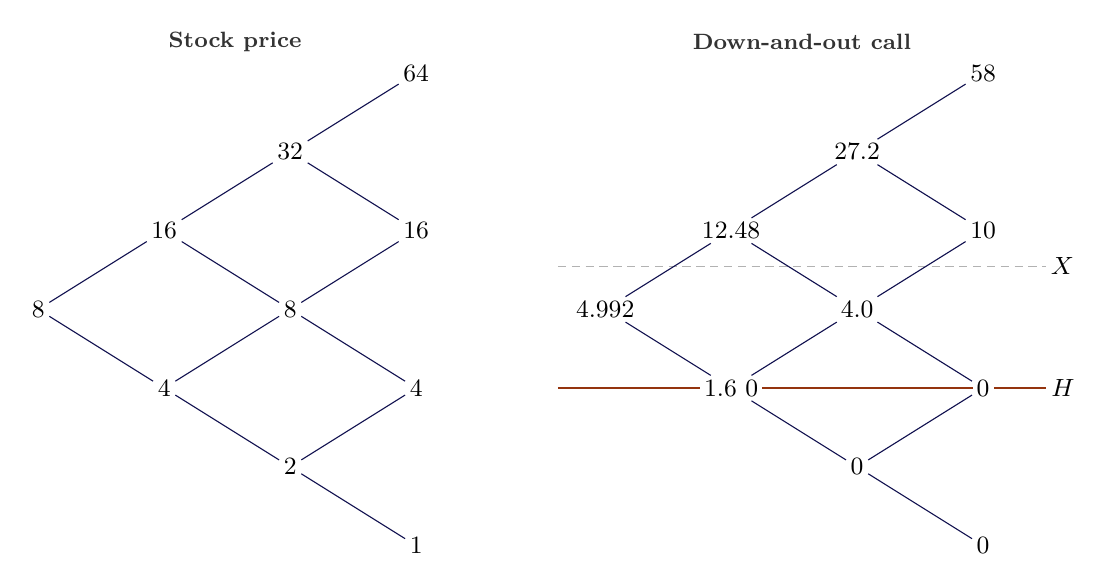
\begin{tikzpicture}[font=\small, every node/.style={inner sep=1.5pt},
			ln/.style={MidnightBlue!70!black}]
		\begin{scope}
			\node[font=\footnotesize\bfseries, text=Gray!40!black] at (2.5,3.4) {Stock price};
			\node (a) at (0,0) {$8$};
			\node (b0) at (1.6,1) {$16$}; \node (b1) at (1.6,-1) {$4$};
			\node (c0) at (3.2,2) {$32$}; \node (c1) at (3.2,0) {$8$}; \node (c2) at (3.2,-2) {$2$};
			\node (d0) at (4.8,3) {$64$}; \node (d1) at (4.8,1) {$16$}; \node (d2) at (4.8,-1) {$4$}; \node (d3) at (4.8,-3) {$1$};
			\foreach \x/\y in {a/b0,a/b1,b0/c0,b0/c1,b1/c1,b1/c2,c0/d0,c0/d1,c1/d1,c1/d2,c2/d2,c2/d3} \draw[ln] (\x)--(\y);
		\end{scope}
		\begin{scope}[xshift=7.2cm]
			\node[font=\footnotesize\bfseries, text=Gray!40!black] at (2.5,3.4) {Down-and-out call};
			\draw[Gray!60, densely dashed] (-0.6,0.55) -- (5.6,0.55) node[right, text=black] {$X$};
			\draw[RawSienna, thick] (-0.6,-1) -- (5.6,-1) node[right, text=black] {$H$};
			\node (a) at (0,0) {$4.992$};
			\node (b0) at (1.6,1) {$12.48$}; \node[fill=white] (b1) at (1.6,-1) {$\cancel{1.6}\ 0$};
			\node (c0) at (3.2,2) {$27.2$}; \node (c1) at (3.2,0) {$4.0$}; \node (c2) at (3.2,-2) {$0$};
			\node (d0) at (4.8,3) {$58$}; \node (d1) at (4.8,1) {$10$}; \node[fill=white] (d2) at (4.8,-1) {$0$}; \node (d3) at (4.8,-3) {$0$};
			\foreach \x/\y in {a/b0,a/b1,b0/c0,b0/c1,b1/c1,b1/c2,c0/d0,c0/d1,c1/d1,c1/d2,c2/d2,c2/d3} \draw[ln] (\x)--(\y);
		\end{scope}
	\end{tikzpicture}
	\caption{\autoref{eg:down-and-out-tree}. Nodes on or below $H=4$ are set to
		zero. ($X=6$ falls between the stock prices $4$ and $8$; the dashed line is only
		schematic.)}
	\label{fig:down-and-out-tree}
\end{figure}

\zh{圖：$H=4$ 以下（含）的 node 設為 $0$。}

\begin{algorithm}[H]
	\caption{Binomial tree algorithm for down-and-out calls on a non-dividend-paying stock}
	\label{alg:down-and-out}
	\KwIn{$S,u,d,X,H,n,\hat{r}$ \quad ($H<X$, $H<S$, $ud=1$)}
	$R:=e^{\hat{r}}$\; $p:=(R-d)/(u-d)$\;
	$h:=\lfloor\ln(H/S)/\ln u\rfloor$\tcp*{effective barrier $Su^{h}\le H$}
	\For{$i=0,1,\ldots,n$}{
		$C[\,i\,]:=\max\bigl(0,\,Su^{n-i}d^{i}-X\bigr)$\;
	}
	\If{$n-h$ is even and $0\le(n-h)/2\le n$}{$C[\,(n-h)/2\,]:=0$\tcp*{a hit}}
	\For{$j=n-1$ \KwTo $0$}{
		\For{$i=0,1,\ldots,j$}{
			$C[\,i\,]:=\bigl(p\times C[\,i\,]+(1-p)\times C[\,i+1\,]\bigr)/R$\;
		}
		\If{$j-h$ is even and $0\le(j-h)/2\le j$}{$C[\,(j-h)/2\,]:=0$\tcp*{a hit}}
	}
	\Return{$C[\,0\,]$}\;
\end{algorithm}

\zh{演算法：$ud=1$，$h=\lfloor\ln(H/S)/\ln u\rfloor$ 是 effective barrier $Su^{h}\le H$ 的層數；每一欄做完 backward induction，就把剛好在 barrier 那層的 node 設成 $0$。}

\begin{note}
	\textbf{$h$ 是什麼。}因為 $ud=1$，tree 上所有股價都是 $Su^{k}$（$k$ 為整數）。effective barrier 是 $\le H$ 的最高那一層：$Su^{k}\le H\iff k\le\ln(H/S)/\ln u$，取最大的整數 $k$ 就是 $h=\lfloor\ln(H/S)/\ln u\rfloor$。
	\textbf{哪個 node 是 barrier。}時間 $j$ 時經過 $i$ 次下跌的節點價格為 $Su^{(j-i)-i}=Su^{j-2i}$，它等於 $Su^{h}$ 恰好在 $j-2i=h$，即 $i=(j-h)/2$。$i$ 必須是 $0$ 到 $j$ 之間的整數，所以演算法要檢查 $j-h$ 是偶數且 $0\le(j-h)/2\le j$。
	只要把那個節點設為零就夠了：它下面的每個節點都只能經由 barrier 那一層到達，而那裡的值已經是 $0$。
	若有 rebate $K$，就把那個節點設成 $K$ 而不是 $0$。\footnote{課本 Figure 11.4。}
\end{note}

\source{Slides pp.~411--412}

But convergence is erratic, because $H$ is not at a price level on the tree.\footnote{Boyle \& Lau (1994).}
The barrier $H$ is moved lower (or higher, if you so choose) to the nearest node price, and this \vocab{effective barrier} changes as $n$ increases.
In fact, the binomial tree is only $O(1/\sqrt{n})$ convergent.\footnote{Tavella \& Randall (2000); J.~Lin (\texttt{R95221010}) (2008); J.~Lin (\texttt{R95221010}) \& Palmer (2013).}
Solutions will be presented later.

\zh{但收斂不規則，因為 $H$ 通常不在 tree 的價格層上：$H$ 被移到最近的 node 價格（effective barrier），而它會隨 $n$ 改變。事實上 binomial tree 只有 $O(1/\sqrt{n})$ 的收斂速度，解法之後再談。}

\begin{figure}[H]
	\centering
	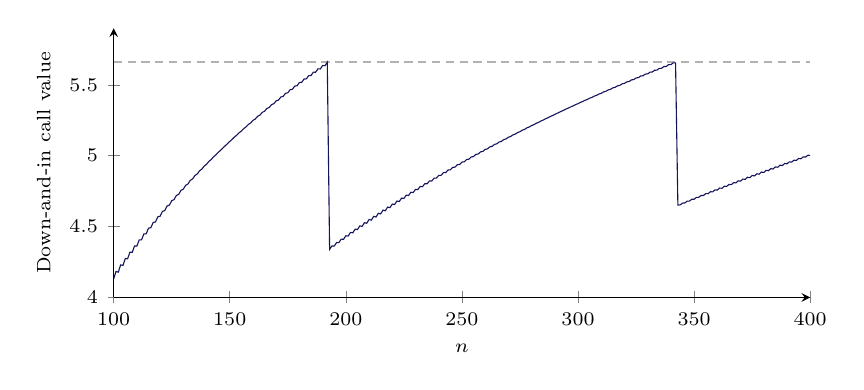
\begin{tikzpicture}[font=\footnotesize]
		\begin{axis}[
				width=0.86\textwidth, height=5.0cm,
				xmin=100, xmax=400, ymin=4.0, ymax=5.9,
				xlabel={$n$}, ylabel={Down-and-in call value},
				axis lines=left, axis line style={thin},
				label style={font=\scriptsize}, tick label style={font=\scriptsize},
			]
			\addplot[Gray!60, thick, densely dashed] coordinates {(100,5.6605) (400,5.6605)};
			\addplot[MidnightBlue!80!black, thin] coordinates {(100,4.1296) (101,4.1832) (102,4.1782) (103,4.2295) (104,4.2257) (105,4.2749) (106,4.2723) (107,4.3193) (108,4.3179) (109,4.3629) (110,4.3625) (111,4.4056) (112,4.4063) (113,4.4475) (114,4.4492) (115,4.4886) (116,4.4912) (117,4.5288) (118,4.5325) (119,4.5684) (120,4.5729) (121,4.6072) (122,4.6126) (123,4.6453) (124,4.6516) (125,4.6827) (126,4.6899) (127,4.7195) (128,4.7275) (129,4.7556) (130,4.7644) (131,4.7911) (132,4.8006) (133,4.8260) (134,4.8363) (135,4.8603) (136,4.8713) (137,4.8940) (138,4.9057) (139,4.9272) (140,4.9395) (141,4.9598) (142,4.9728) (143,4.9919) (144,5.0056) (145,5.0235) (146,5.0378) (147,5.0546) (148,5.0695) (149,5.0852) (150,5.1007) (151,5.1154) (152,5.1314) (153,5.1451) (154,5.1616) (155,5.1743) (156,5.1914) (157,5.2031) (158,5.2207) (159,5.2315) (160,5.2496) (161,5.2594) (162,5.2781) (163,5.2870) (164,5.3061) (165,5.3142) (166,5.3337) (167,5.3409) (168,5.3610) (169,5.3673) (170,5.3878) (171,5.3934) (172,5.4143) (173,5.4191) (174,5.4404) (175,5.4444) (176,5.4661) (177,5.4694) (178,5.4915) (179,5.4941) (180,5.5166) (181,5.5184) (182,5.5413) (183,5.5424) (184,5.5657) (185,5.5661) (186,5.5897) (187,5.5895) (188,5.6135) (189,5.6126) (190,5.6369) (191,5.6354) (192,5.6600) (193,4.3386) (194,4.3631) (195,4.3626) (196,4.3873) (197,4.3863) (198,4.4113) (199,4.4098) (200,4.4351) (201,4.4330) (202,4.4585) (203,4.4559) (204,4.4818) (205,4.4787) (206,4.5047) (207,4.5011) (208,4.5275) (209,4.5234) (210,4.5500) (211,4.5454) (212,4.5722) (213,4.5672) (214,4.5942) (215,4.5893) (216,4.6160) (217,4.6115) (218,4.6376) (219,4.6335) (220,4.6589) (221,4.6553) (222,4.6801) (223,4.6768) (224,4.7010) (225,4.6981) (226,4.7217) (227,4.7193) (228,4.7422) (229,4.7402) (230,4.7625) (231,4.7608) (232,4.7826) (233,4.7813) (234,4.8025) (235,4.8016) (236,4.8222) (237,4.8217) (238,4.8417) (239,4.8416) (240,4.8611) (241,4.8613) (242,4.8802) (243,4.8808) (244,4.8992) (245,4.9001) (246,4.9180) (247,4.9193) (248,4.9366) (249,4.9382) (250,4.9551) (251,4.9570) (252,4.9734) (253,4.9756) (254,4.9915) (255,4.9941) (256,5.0094) (257,5.0123) (258,5.0272) (259,5.0305) (260,5.0449) (261,5.0484) (262,5.0623) (263,5.0662) (264,5.0797) (265,5.0838) (266,5.0968) (267,5.1013) (268,5.1139) (269,5.1186) (270,5.1307) (271,5.1357) (272,5.1475) (273,5.1528) (274,5.1641) (275,5.1696) (276,5.1805) (277,5.1863) (278,5.1968) (279,5.2029) (280,5.2130) (281,5.2194) (282,5.2290) (283,5.2356) (284,5.2449) (285,5.2518) (286,5.2607) (287,5.2678) (288,5.2764) (289,5.2837) (290,5.2919) (291,5.2995) (292,5.3073) (293,5.3151) (294,5.3225) (295,5.3306) (296,5.3377) (297,5.3460) (298,5.3527) (299,5.3613) (300,5.3676) (301,5.3764) (302,5.3824) (303,5.3914) (304,5.3971) (305,5.4063) (306,5.4116) (307,5.4211) (308,5.4261) (309,5.4357) (310,5.4404) (311,5.4503) (312,5.4547) (313,5.4647) (314,5.4688) (315,5.4791) (316,5.4828) (317,5.4933) (318,5.4967) (319,5.5074) (320,5.5105) (321,5.5214) (322,5.5242) (323,5.5353) (324,5.5378) (325,5.5490) (326,5.5513) (327,5.5627) (328,5.5647) (329,5.5763) (330,5.5780) (331,5.5898) (332,5.5912) (333,5.6032) (334,5.6043) (335,5.6165) (336,5.6173) (337,5.6297) (338,5.6302) (339,5.6428) (340,5.6431) (341,5.6558) (342,5.6558) (343,4.6522) (344,4.6529) (345,4.6658) (346,4.6663) (347,4.6794) (348,4.6796) (349,4.6929) (350,4.6928) (351,4.7062) (352,4.7060) (353,4.7195) (354,4.7190) (355,4.7327) (356,4.7320) (357,4.7459) (358,4.7449) (359,4.7589) (360,4.7577) (361,4.7719) (362,4.7705) (363,4.7847) (364,4.7831) (365,4.7975) (366,4.7957) (367,4.8102) (368,4.8082) (369,4.8229) (370,4.8206) (371,4.8354) (372,4.8330) (373,4.8479) (374,4.8453) (375,4.8603) (376,4.8575) (377,4.8727) (378,4.8696) (379,4.8849) (380,4.8817) (381,4.8971) (382,4.8940) (383,4.9092) (384,4.9063) (385,4.9212) (386,4.9186) (387,4.9332) (388,4.9307) (389,4.9451) (390,4.9428) (391,4.9569) (392,4.9548) (393,4.9687) (394,4.9668) (395,4.9804) (396,4.9786) (397,4.9920) (398,4.9904) (399,5.0035) (400,5.0022)};
		\end{axis}
	\end{tikzpicture}
	\caption{CRR binomial values of the down-and-in call of \autoref{fig:down-and-in}
		($S=95$, $X=100$, $H=90$, $r=10\%$, $\sigma=25\%$, $\tau=1$), computed by
		in--out parity, for $n=100,\ldots,400$. Dashed: the analytical value
		$5.6605$. Each jump down happens when the effective barrier moves to the
		next lattice level; in between the value creeps up with an odd--even
		wobble. Cf.\ Lyuu (1998).}
	\label{fig:barrier-convergence}
\end{figure}

\zh{圖：\autoref{fig:down-and-in} 的 down-and-in call（$S=95$）用 CRR tree 加 in--out parity 計算，$n=100$ 到 $400$；虛線是解析值 5.6605。effective barrier 每移到下一層，數值就往下跳；之間慢慢上升並有奇偶擺動。}

\begin{intuition}
	The effective barrier $Su^{h}$ sits below $H$ by a random-looking fraction of one step $\sigma\sqrt{\Delta t}$.
	A barrier misplaced by $O(\sqrt{\Delta t})=O(1/\sqrt{n})$ shifts the knock-in probability by the same order, and that is the error.
	As $n$ grows the lattice level just below $H$ creeps up towards $H$, the value rises, until a new level appears below $H$ and the effective barrier drops back --- the saw-tooth.
	The cure is to choose $n$ (or shift the lattice) so that $H$ falls exactly on a node.
\end{intuition}

\zh{effective barrier $Su^{h}$ 比 $H$ 低了一步 $\sigma\sqrt{\Delta t}$ 中看似隨機的一部分；barrier 放錯 $O(1/\sqrt{n})$，knock-in 機率就差同樣的量級，這就是誤差。$n$ 增加時 $H$ 下方那層慢慢靠近 $H$、數值上升，直到 $H$ 下方出現新的一層、effective barrier 又掉下去——形成鋸齒。解法是選 $n$（或平移 lattice）讓 $H$ 落在 node 上。}

\subsection{Other Types of Barrier Options}

\source{Slide p.~413}

Partial barrier options (the barrier is active during only an initial period), forward-starting barrier options (only the latter part), window barrier options, rolling barrier options,\footnote{The barrier is a step function. There is a pricing formula as a multiple integral (H.~Lee, G.~Lee, \& Song, 2022). There is also an $O(n\ln n)$-time tree algorithm by Y.~Lu (\texttt{R06723032}, \texttt{D08922008}) and Lyuu (2021, 2023).} and moving barrier options.\footnote{Armstrong (2001); Carr \& A.~Chou (1997); Davydov \& Linetsky (2001/2002); Haug (1998).}

\zh{其他種類：partial barrier（只在開始一段時間有效）、forward-starting barrier（只在後段有效）、window barrier、rolling barrier（barrier 是階梯函數）、moving barrier。}

\subsection{Daily Monitoring}

\source{Slides pp.~414--416}

Many barrier options monitor the barrier only for daily closing prices.
If so, only nodes at the end of a day need to check for the barrier condition.
We can even remove intraday nodes to create a \vocab{multinomial tree}: a node is then followed by $d+1$ nodes if each day is partitioned into $d$ periods (\autoref{fig:heptanomial}), with branching probabilities $b(j;d,p)$.

\zh{很多 barrier option 只用每天收盤價檢查 barrier，所以只有每天結束的 node 需要檢查。甚至可以拿掉盤中 node 變成 multinomial tree：一天切成 $d$ 期時，每個 node 接 $d+1$ 個 node，分支機率是 $b(j;d,p)$。}

\begin{figure}[H]
	\centering
	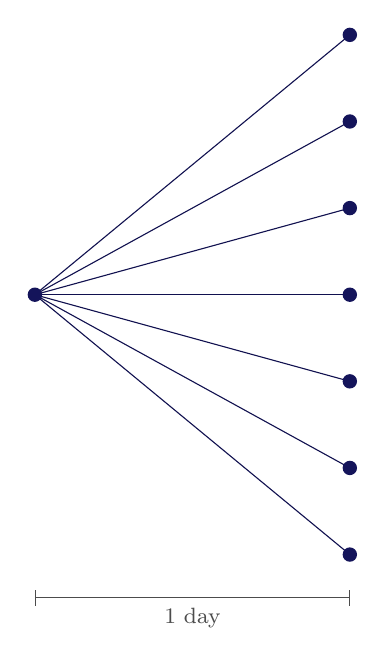
\begin{tikzpicture}[x=1cm, y=0.55cm]
		\foreach \k in {-3,...,3} {
				\draw[MidnightBlue!70!black] (0,0) -- (4,2*\k/1);
				\fill[MidnightBlue!80!black] (4,2*\k/1) circle (2.6pt);
			}
		\fill[MidnightBlue!80!black] (0,0) circle (2.6pt);
		\draw[|-|, Gray!60!black] (0,-7) -- (4,-7) node[midway, below, font=\footnotesize] {1 day};
	\end{tikzpicture}
	\caption{A heptanomial tree: 6 periods per day, intraday nodes removed. The
		seven successors are the end-of-day prices $Su^{6-2j}$, $j=0,\ldots,6$.}
	\label{fig:heptanomial}
\end{figure}

\zh{圖：heptanomial tree：一天 6 期、拿掉盤中 node，七個後繼是當天收盤價 $Su^{6-2j}$，$j=0,\ldots,6$。}

Does this save time or space?\footnote{Contributed by Ms.~Chen, Tzu-Chun (\texttt{R94922003}) and others on April 12, 2006.}
Not asymptotically.
Over $D$ days with $d$ periods each, the binomial tree visits $\sim(Dd)^{2}/2$ nodes at two operations each, about $D^{2}d^{2}$ operations; the multinomial tree visits only the $\sim D^{2}d/2$ end-of-day nodes but at $d+1$ operations each, again of order $D^{2}d^{2}/2$.
Space is a single column of $O(Dd)$ nodes either way.

\zh{這樣能省時間或空間嗎？漸近上不能：binomial tree 約 $(Dd)^{2}/2$ 個 node、每個 2 次運算；multinomial tree 只有約 $D^{2}d/2$ 個收盤 node、但每個 $d+1$ 次運算，都是 $D^{2}d^{2}$ 的量級。空間都是一欄 $O(Dd)$。}

\begin{remark}
	\begin{enumerate}[(1),nosep]
		\item \textbf{multinomial 的分支機率。}一天有 $d$ 期，一天後股價由這 $d$ 期中上漲幾次決定：上漲 $j$ 次（$j=0,\ldots,d$）共 $d+1$ 種結果，機率是 $b(j;d,p)$（\autoref{sec:bopm-formula} 的 binomial distribution）。
		\item \textbf{binomial tree 的工作量。}總共 $Dd$ 期，node 數 $\sum_{k=0}^{Dd}(k+1)\sim(Dd)^{2}/2$，每個 node 合併 $2$ 個子節點。
		\item \textbf{multinomial tree 的工作量。}只留每天結束時的 node：第 $k$ 天結束時有 $kd+1$ 個，總共 $\sum_{k=0}^{D}(kd+1)\sim dD^{2}/2$ 個；但每個 node 要合併 $d+1$ 個子節點，總共 $\sim dD^{2}/2\times d=D^{2}d^{2}/2$。
	\end{enumerate}
	兩者同為 $O(D^{2}d^{2})$，所以沒有省下。
\end{remark}

\paragraph{Discrete versus continuous monitoring.}
Discrete barriers are more expensive for knock-out options than continuous ones, and less expensive for knock-in options --- a path can cross $H$ between two closes without being seen.
Discrete barriers are far less popular than continuous ones for individual stocks; they are equally popular for indices.\footnote{Bennett (2014).}

\zh{discrete 與 continuous monitoring：knock-out 的 discrete barrier 比 continuous 貴、knock-in 則比較便宜，因為路徑可能在兩次收盤之間穿過 $H$ 而沒被看到。個股上 discrete barrier 遠不如 continuous 普及，指數上則一樣普及。}

%─────§ Foreign currencies──────────────────────────────────────────────────────────────────────────────────────────────────────────────────────────
\section{Foreign Currencies}
\label{sec:forex}

\source{Slides pp.~417--419}

\begin{flushright}
	\itshape Data! data! data!\\
	\upshape --- Arthur Conan Doyle (1892), \itshape The Adventures of Sherlock Holmes
\end{flushright}

\begin{notation}
	\begin{itemize}[nosep]
		\item $S$: the spot exchange rate in domestic/foreign terms, i.e., the number of domestic currencies per unit of foreign currency;\footnote{The market convention is the opposite: A/B $=x$ means one unit of currency A (the reference or base currency) is equal to $x$ units of currency B (the counter-value currency).}
		\item $\sigma$: the volatility of the exchange rate;
		\item $r$: the domestic interest rate;
		\item $r_{f}$: the foreign interest rate. (The slides write $\hat{r}$; we keep $\hat{r}$ for the per-period rate of \autoref{sec:pricing-setting}.)
	\end{itemize}
\end{notation}

\zh{$S$ 是匯率（一單位外幣值多少本國貨幣），$\sigma$ 是匯率波動率，$r$ 是本國利率，$r_{f}$ 是外國利率。}

A foreign currency is analogous to a stock paying a known dividend yield: holding foreign currency means holding foreign bonds, which pay a ``continuous dividend yield'' equal to $r_{f}$ in the foreign currency.

\zh{外幣就像有已知 dividend yield 的股票：持有外幣等於持有外國債券，會以 $r_{f}$ 的「連續股利」生出外幣。}

\begin{remark}
	站在本國投資人的角度，持有一單位外幣（存在外國銀行）會以利率 $r_{f}$ 連續生出更多外幣，就像股票以殖利率 $q$ 連續配息。所以 \autoref{sec:continuous-yield} 的所有結果，把 $q$ 換成 $r_{f}$ 就能直接用。
\end{remark}

\source{Slides pp.~420--429, 435--437}

The slides then plot daily and minutely Euro--USD and GBP--USD rates (2005--2017), the distribution of GBP--USD between the collapse of Lehman Brothers and the Brexit referendum (September 15, 2008--June 23, 2016), and the daily JPY--USD rate, with their log returns.
As for stocks (\autoref{fig:sp500-density}), the log returns have sharper peaks and heavier tails than the normal --- most visibly at the minute scale --- and the volatility clusters in time.

\zh{簡報畫了 2005--2017 年 Euro--USD、GBP--USD 的日資料和分鐘資料、雷曼倒閉到脫歐公投之間 GBP--USD 的分布、JPY--USD 的日匯率和 log return。和股票一樣，log return 的峰比 normal 尖、尾巴比 normal 厚（分鐘資料最明顯），而且波動在時間上會聚集。}

\subsection{Foreign Exchange Options}

\source{Slide p.~430}

In 2000 the total notional volume of foreign exchange options was US\$13 trillion:\footnote{Lipton (2002).}
\begin{itemize}[nosep]
	\item 38.5\% were vanilla calls and puts with a maturity less than one month;
	\item 52.5\% were vanilla calls and puts with a maturity between one and 18 months;
	\item 4\% were barrier options (\autoref{sec:barrier});
	\item 1.5\% were vanilla calls and puts with a maturity more than 18 months;
	\item 1\% were binary options (\autoref{sec:binary-call});
	\item 0.7\% were Asian options (\autoref{sec:path-dependent}).
\end{itemize}

\zh{2000 年外匯選擇權名目總額 13 兆美元：一個月內到期的普通 call/put 占 38.5\%，一到十八個月 52.5\%，barrier 4\%，十八個月以上 1.5\%，binary 1\%，Asian 0.7\%。}

\source{Slides pp.~431--433}

Foreign exchange options are settled via delivery of the underlying currency, and a primary use of them is to hedge currency risk.

\zh{外匯選擇權以交割標的貨幣結算，主要用途是規避匯率風險。}

\begin{eg}
	A U.S.\ company expects to receive 100 million Japanese yen in March 2000, to be exchanged for U.S.\ dollars.
	The contract size for the Japanese yen option is JPY6,250,000, so the company purchases
	\[
		\frac{100{,}000{,}000}{6{,}250{,}000} \;=\; 16
	\]
	puts on the Japanese yen with a strike of \$.0088/JPY1 and an exercise month in March 2000.
	This put is in the money if the JPY--USD exchange rate drops below 0.0088, and it gives the company the right to sell 100,000,000 Japanese yen for $100{,}000{,}000\times.0088=880{,}000$ U.S.\ dollars.
\end{eg}

\zh{例子：美國公司預計 2000 年 3 月收到 1 億日圓並換成美元。日圓選擇權每口 625 萬日圓，所以買 16 口 strike 0.0088 美元/日圓、3 月到期的 put。JPY--USD 跌破 0.0088 時 put 在價內，公司有權把 1 億日圓以 880{,}000 美元賣出。}

Note that these puts are equivalent to the right to \emph{buy} 880,000 U.S.\ dollars with 100,000,000 Japanese yen.
From this angle, they become calls --- on the dollar, with strike $1/0.0088\approx113.6$ yen per dollar.
A put on one currency is a call on the other.

\zh{這些 put 等於用 1 億日圓買 880{,}000 美元的權利，換個角度就是美元的 call，strike $1/0.0088\approx113.6$ 日圓/美元：一種貨幣的 put 就是另一種貨幣的 call。}

\begin{remark}
	「用 100M JPY 換 880K USD 的權利」從美元的角度看，就是「付 100M JPY 買 880K USD 的權利」。strike 改用「每美元幾日圓」表示是 $100{,}000{,}000/880{,}000=1/0.0088\approx113.6$。日圓貶值（JPY--USD $<0.0088$）等價於美元升值（USD--JPY $>113.6$），所以 yen put 在價內時，dollar call 也在價內。
\end{remark}

\subsection{The Black--Scholes Model for Forex Options}

\source{Slide p.~434}

Assume the exchange rate $S$ is lognormally distributed.
The formulas \eqref{eq:bs-call-q}--\eqref{eq:bs-put-q} apply with the dividend yield equal to $r_{f}$:
\begin{align}
	C & \;=\; Se^{-r_{f}\tau}N(x)-Xe^{-r\tau}N\bigl(x-\sigma\sqrt{\tau}\bigr) , \label{eq:forex-call} \\
	P & \;=\; Xe^{-r\tau}N\bigl(-x+\sigma\sqrt{\tau}\bigr)-Se^{-r_{f}\tau}N(-x) , \label{eq:forex-put}
\end{align}
where
\[
	x \;\triangleq\; \frac{\ln(S/X)+\bigl(r-r_{f}+\sigma^{2}/2\bigr)\tau}{\sigma\sqrt{\tau}} .
\]
These are the \vocab{Garman--Kohlhagen} formulas.
On a tree, use the risk-neutral probability \eqref{eq:rn-p-yield} with $q=r_{f}$.

\zh{假設匯率是 lognormal，\eqref{eq:bs-call-q}--\eqref{eq:bs-put-q} 把 dividend yield 換成 $r_{f}$ 即適用，得到 Garman--Kohlhagen 公式；在 tree 上用 \eqref{eq:rn-p-yield}，$q=r_{f}$。}

\begin{note}
	dividend 的類比也把 early exercise 的結論一起帶過來。
	現在 no-arbitrage 下界是 $C\ge\max\bigl(Se^{-r_{f}\tau}-Xe^{-r\tau},0\bigr)$：到期拿到的外幣 $S_{\tau}$ 今天值 $Se^{-r_{f}\tau}$（\autoref{sec:continuous-yield}），要付的 $X$ 今天值 $Xe^{-r\tau}$。
	當 $r_{f}>r$ 時它會\emph{低於} intrinsic value $S-X$：兩者相減
	\[
		(S-X)-\bigl(Se^{-r_{f}\tau}-Xe^{-r\tau}\bigr)=S\bigl(1-e^{-r_{f}\tau}\bigr)-X\bigl(1-e^{-r\tau}\bigr) ,
	\]
	$S\ge X$ 時第一項 $\ge X(1-e^{-r_{f}\tau})>X(1-e^{-r\tau})$，所以差為正。
	所以和 \autoref{thm:merton-no-early} 不同，American forex call 可能會在到期前 early exercise。\footnote{課本 Theorem 11.5.1。}
\end{note}

%─────§ Path-dependent derivatives──────────────────────────────────────────────────────────────────────────────────────────────────────────────────
\section{Path-Dependent Derivatives}
\label{sec:path-dependent}

\source{Slides pp.~438--439}

\begin{flushright}
	\itshape Bar the roads! Bar the paths!\\
	Wert thou to flee from here, wert thou\\
	to find all the roads of the world,\\
	the way thou seekst\\
	the path to that thou'dst find not[.]\\
	\upshape --- Richard Wagner (1813--1883), \itshape Parsifal
\end{flushright}

Let $S_{0},S_{1},\ldots,S_{n}$ denote the prices of the underlying asset over the life of the option; $S_{0}$ is the known price at time zero and $S_{n}$ is the price at expiration.
The standard European call has a terminal value $\max(S_{n}-X,0)$ depending only on the last price, so its value depends only on the underlying asset's terminal price regardless of how it gets there.\footnote{Called \vocab{simple claims} (Björk, 2009).}

\zh{令 $S_{0},\ldots,S_{n}$ 為存續期間的標的價格，$S_{0}$ 是現在、$S_{n}$ 是到期。普通 European call 的 payoff $\max(S_{n}-X,0)$ 只看最後的價格，不管怎麼走到那裡。}

\source{Slides pp.~440--441}

Some derivatives are \vocab{path-dependent}: their terminal payoff depends explicitly on the path.

\zh{有些 derivative 是 path-dependent：payoff 明確取決於整條路徑。}

\begin{definition}
	The (arithmetic) \vocab{average-rate call} and \vocab{average-rate put} have terminal values
	\[
		\max\left(\frac{1}{n+1}\sum_{i=0}^{n}S_{i}-X,\ 0\right) ,
		\qquad
		\max\left(X-\frac{1}{n+1}\sum_{i=0}^{n}S_{i},\ 0\right) .
	\]
\end{definition}

\zh{算術 average-rate call / put 的 payoff 是「平均價格 $-X$」/「$X-$ 平均價格」的正部分。}

Average-rate options are also called \vocab{Asian options}.
They are very popular:\footnote{As of the late 1990s, the outstanding volume was in the range of 5--10 billion U.S.\ dollars (Nielsen \& Sandmann, 2003).} they are useful hedging tools for firms that will make a stream of purchases over a time period, because the costs are likely to be linked to the average price.
They are mostly European for the same reason.
The averaging clause is also common in convertible bonds and structured notes.

\zh{average-rate option 又叫 Asian option，很受歡迎：對一段時間內持續採購的公司是好用的避險工具，因為成本跟平均價格有關；也因此多半是 European。平均條款在可轉債和結構型商品中也很常見。}

\begin{remark}
	\vocab{亞式選擇權}（Asian option）：報酬取決於存續期間股價的\emph{平均}而非到期價。平均比單一價格難操縱、波動也小，因此比歐式選擇權便宜，適合持續採購原料的公司避險。名稱據說來自最早用在亞洲交易量較小的股票上。
\end{remark}

\source{Slides pp.~442--443}

\begin{definition}
	\begin{itemize}[nosep]
		\item A \vocab{lookback call} on the minimum pays $S_{n}-\min_{0\le i\le n}S_{i}$; a \vocab{lookback put} on the maximum pays $\max_{0\le i\le n}S_{i}-S_{n}$.
		\item The \vocab{fixed-strike lookback option} (also called forward lookback option) pays
		      \[
			      \max\Bigl(\max_{0\le i\le n}S_{i}-X,\,0\Bigr)\ \text{(call)},
			      \qquad
			      \max\Bigl(X-\min_{0\le i\le n}S_{i},\,0\Bigr)\ \text{(put)}.
		      \]
		\item Lookback calls and puts on the average (instead of a constant $X$) are called \vocab{average-strike options}.
	\end{itemize}
\end{definition}

\zh{lookback call（對最小值）付 $S_{n}-\min S_{i}$，lookback put（對最大值）付 $\max S_{i}-S_{n}$。fixed-strike lookback 付 $\max(\max S_{i}-X,0)$（call）或 $\max(X-\min S_{i},0)$（put）。strike 換成平均價的 lookback 叫 average-strike option。}

The lookback call lets the holder buy at the lowest price of the period, the lookback put sell at the highest: ``selling at the high and buying at the low.''
The CRR tree converges uniformly for path-dependent options.\footnote{Jiang \& M.~Dai (2004).}

\zh{lookback call 讓持有者以期間最低價買入、lookback put 以最高價賣出：「買在最低、賣在最高」。CRR tree 對 path-dependent option 一致收斂。}

\subsection{Average-Rate Options Are Hard}

\source{Slides pp.~444--447}

Average-rate options are notoriously hard to price.
The binomial tree for the averages does not combine: the paths $(S_{0},S_{0}u,S_{0}u^{2},S_{0}u^{2}d)$ and $(S_{0},S_{0}d,S_{0}du,S_{0}du^{2})$ end at the same price but with different averages, hence different payoffs (\autoref{fig:asian-tree}).

\zh{average-rate option 出了名地難定價：平均價的 tree 不會 recombine，兩條終點同價的路徑平均不同，payoff 也不同（\autoref{fig:asian-tree}）。}

\begin{remark}
	兩條 path 的終點都是 $S_{0}u^{2}d$，但平均分別是 $\frac{S_{0}}{4}(1+u+u^{2}+u^{2}d)$ 和 $\frac{S_{0}}{4}(1+d+du+du^{2})$。$u>d$ 時逐項比較，前者每一項都 $\ge$ 後者，所以平均比較大：先漲的 path 中途價格比較高。
\end{remark}

\begin{figure}[H]
	\centering
	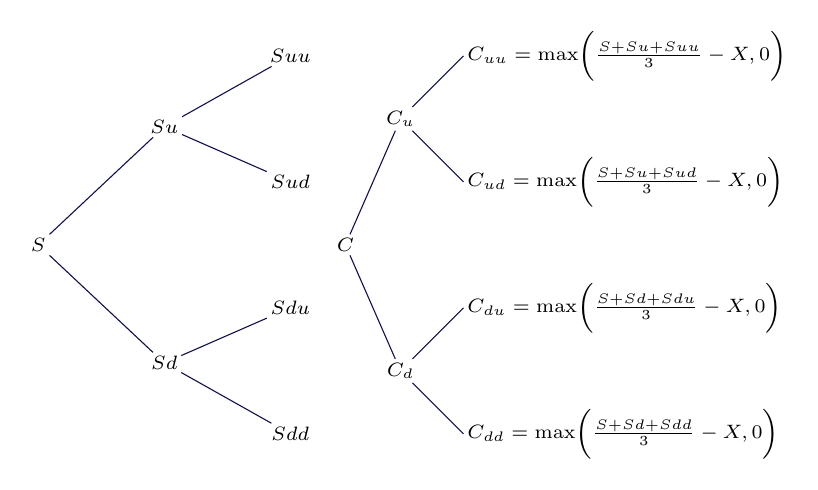
\begin{tikzpicture}[font=\scriptsize, every node/.style={inner sep=1.2pt},
			ln/.style={MidnightBlue!70!black}]
		\node (s) at (0,0) {$S$};
		\node (u) at (1.6,1.5) {$Su$}; \node (d) at (1.6,-1.5) {$Sd$};
		\node (uu) at (3.2,2.4) {$Suu$}; \node (ud) at (3.2,0.8) {$Sud$};
		\node (du) at (3.2,-0.8) {$Sdu$}; \node (dd) at (3.2,-2.4) {$Sdd$};
		\foreach \x/\y in {s/u,s/d,u/uu,u/ud,d/du,d/dd} \draw[ln] (\x)--(\y);
		\node[anchor=west] (cuu) at (5.4,2.4) {$C_{uu}=\max\bigl(\frac{S+Su+Suu}{3}-X,0\bigr)$};
		\node[anchor=west] (cud) at (5.4,0.8) {$C_{ud}=\max\bigl(\frac{S+Su+Sud}{3}-X,0\bigr)$};
		\node[anchor=west] (cdu) at (5.4,-0.8) {$C_{du}=\max\bigl(\frac{S+Sd+Sdu}{3}-X,0\bigr)$};
		\node[anchor=west] (cdd) at (5.4,-2.4) {$C_{dd}=\max\bigl(\frac{S+Sd+Sdd}{3}-X,0\bigr)$};
		\node (cu) at (4.6,1.6) {$C_{u}$}; \node (cd) at (4.6,-1.6) {$C_{d}$};
		\node (c) at (3.9,0) {$C$};
		\draw[ln] (c)--(cu); \draw[ln] (c)--(cd);
		\draw[ln] (cu)--(cuu.west); \draw[ln] (cu)--(cud.west);
		\draw[ln] (cd)--(cdu.west); \draw[ln] (cd)--(cdd.west);
	\end{tikzpicture}
	\caption{Two periods of an average-rate call. The stock tree on the left
		recombines ($Sud=Sdu$); the pricing tree on the right does not, since
		$C_{ud}\ne C_{du}$ in general. With $C_{u}=\bigl[pC_{uu}+(1-p)C_{ud}\bigr]/e^{\hat{r}}$
		and similarly for $C_{d}$ and $C$, the pricing tree grows exponentially.}
	\label{fig:asian-tree}
\end{figure}

\zh{圖：兩期的 average-rate call。左邊股價 tree 會 recombine（$Sud=Sdu$），右邊定價 tree 不會，因為一般 $C_{ud}\ne C_{du}$；定價 tree 呈指數成長。}

A naive algorithm enumerates the $2^{n}$ paths for an $n$-period binomial tree and then averages the payoffs, but the complexity is exponential.\footnote{T.~Dai (\texttt{B82506025}, \texttt{R86526008}, \texttt{D8852600}) \& Lyuu (2007) reduce it to $2^{O(\sqrt{n})}$.}
The Monte Carlo method and approximation algorithms are some of the alternatives left.

\zh{天真的演算法列舉 $2^{n}$ 條路徑再平均 payoff，是指數時間；剩下的選擇有 Monte Carlo 和近似演算法。}

\paragraph{States and their transitions.}
The tuple $(i,S,P)$ captures the state for the Asian option --- a ``sufficient statistic,'' if you will --- where $i$ is the time, $S$ the prevailing stock price, and $P$ the running sum.\footnote{When the average is a moving average, a different technique is needed (C.~Kao (\texttt{R89723057}) \& Lyuu, 2003).}
For the binomial model the state transition is
\[
	(i,S,P) \;\longrightarrow\;
	\begin{cases}
		(i+1,\,Su,\,P+Su), & \text{for the up move},   \\
		(i+1,\,Sd,\,P+Sd), & \text{for the down move}.
	\end{cases}
\]
The number of states is exponential: $(i,S)$ takes $O(n^{2})$ values, but the running sum $P$ distinguishes paths.

\zh{$(i,S,P)$ 足以描述 Asian option 的狀態（時間、股價、累積和）。上漲變成 $(i+1,Su,P+Su)$，下跌變成 $(i+1,Sd,P+Sd)$。$(i,S)$ 只有 $O(n^{2})$ 種，但累積和 $P$ 會區分不同路徑，所以狀態數是指數的。}

\begin{remark}
	關鍵在於「狀態」要包含哪些資訊才足以決定未來報酬。歐式選擇權只需要 $(i,S)$，所以二項樹會重合；亞式選擇權還需要目前的累積和 $P$，而不同路徑到同一個 $(i,S)$ 幾乎都有不同的 $P$，樹就不再重合。
\end{remark}

\subsection{Geometric Averages}

\source{Slides pp.~448--449}

Not all path-dependent derivatives are hard to price; barrier options are easy, for example.
When averaging is done geometrically, the option payoffs are
\[
	\max\Bigl((S_{0}S_{1}\cdots S_{n})^{1/(n+1)}-X,\ 0\Bigr) ,
	\qquad
	\max\Bigl(X-(S_{0}S_{1}\cdots S_{n})^{1/(n+1)},\ 0\Bigr) .
\]

\begin{theorem}[Angus, 1999]
	\label{thm:geometric-asian}
	The limiting analytical solutions are the Black--Scholes formulas
	\begin{align}
		C & \;=\; Se^{-q_{a}\tau}N(x)-Xe^{-r\tau}N\bigl(x-\sigma_{a}\sqrt{\tau}\bigr) , \label{eq:geo-call} \\
		P & \;=\; Xe^{-r\tau}N\bigl(-x+\sigma_{a}\sqrt{\tau}\bigr)-Se^{-q_{a}\tau}N(-x) , \notag
	\end{align}
	with the volatility set to $\sigma_{a}\triangleq\sigma/\sqrt{3}$, the dividend yield set to $q_{a}\triangleq(r+q+\sigma^{2}/6)/2$, and
	\[
		x \;\triangleq\; \frac{\ln(S/X)+\bigl(r-q_{a}+\sigma_{a}^{2}/2\bigr)\tau}{\sigma_{a}\sqrt{\tau}} .
	\]
\end{theorem}

\zh{不是所有 path-dependent derivative 都難（barrier 就很容易）。用幾何平均時，payoff 是上面兩式；極限下的解就是 Black--Scholes 公式，只要把波動率換成 $\sigma_{a}=\sigma/\sqrt{3}$、dividend yield 換成 $q_{a}=(r+q+\sigma^{2}/6)/2$。}

\begin{proof}[Proof（補充；簡報只給結論）]
	想法：$\ln G$ 是 normal，算出它的平均和變異數，再找一支「假想股票」讓它的 $\ln S_{\tau}$ 有相同的分布，就能直接套 Black--Scholes。
	\begin{enumerate}[(1),nosep]
		\item \textbf{寫成 normal 的和。}$\ln S_{i}=\ln S_{0}+\sum_{k=1}^{i}\varepsilon_{k}$，在 risk-neutral 下（極限時）$\varepsilon_{k}$ i.i.d.\ $N(m\Delta t,\ \sigma^{2}\Delta t)$，$m\triangleq r-q-\sigma^{2}/2$（\autoref{lem:rn-lognormal}）。
		\item \textbf{交換求和順序。}$\varepsilon_{k}$ 出現在所有 $i\ge k$ 的 $\ln S_{i}$ 裡，共 $n-k+1$ 次，所以
		\[
			\ln G\triangleq\frac{1}{n+1}\sum_{i=0}^{n}\ln S_{i}=\ln S_{0}+\sum_{k=1}^{n}\frac{n-k+1}{n+1}\,\varepsilon_{k} ,
		\]
		是獨立 normal 的加權和，所以也是 normal（\autoref{cor:normal-closure}）。
		\item \textbf{平均。}$\sum_{k=1}^{n}(n-k+1)=\frac{n(n+1)}{2}$，所以 $E[\ln G]-\ln S_{0}=m\Delta t\cdot\frac n2=\frac{m\tau}{2}$。
		\item \textbf{變異數。}$\sum_{k=1}^{n}(n-k+1)^{2}=\frac{n(n+1)(2n+1)}{6}$，所以 $\Var[\ln G]=\sigma^{2}\tau\cdot\frac{2n+1}{6(n+1)}\to\frac{\sigma^{2}\tau}{3}$。
		\item \textbf{對到 Black--Scholes。}dividend yield $q_{a}$、volatility $\sigma_{a}$ 的股票有 $\ln S_{\tau}\sim N\bigl(\ln S+(r-q_{a}-\sigma_{a}^{2}/2)\tau,\ \sigma_{a}^{2}\tau\bigr)$。令它和 $\ln G$ 同分布：$\sigma_{a}^{2}=\sigma^{2}/3$，且 $r-q_{a}-\frac{\sigma^{2}}{6}=\frac m2$，解得 $q_{a}=\frac{r+q}{2}+\frac{\sigma^{2}}{12}=\frac{r+q+\sigma^{2}/6}{2}$。call 價值只由 $G$ 的分布決定，所以 \eqref{eq:bs-call-q} 代入 $q_{a},\sigma_{a}$ 就是答案。
	\end{enumerate}
\end{proof}

See the textbook for a proof based on the binomial model.
Note that $\sigma_{a}<\sigma$: averaging cancels part of the noise, which is why average-rate options are cheaper than their vanilla counterparts.

\zh{二項模型下的證明見課本。注意 $\sigma_{a}<\sigma$：平均會抵銷一部分雜訊，所以 average-rate option 比普通 option 便宜。}

\begin{note}
	geometric average 之所以好算，正是因為 $\ln G$ 是 log return 的\emph{線性}函數，而 normal 的和仍是 normal。
	arithmetic average $\frac1{n+1}\sum S_{i}$ 是一堆 \emph{lognormal} 的和，它不是 lognormal，也沒有 closed-form 的分布。
	實務上，average-rate options 幾乎都使用 arithmetic average。
\end{note}

\subsection{An Approximate Formula for Asian Calls}

\source{Slide p.~450}

For the continuously sampled arithmetic average there is an accurate approximation:\footnote{Rogers \& Shi (1995); Thompson (1999); K.~Chen (\texttt{R92723061}) (2005); K.~Chen (\texttt{R92723061}) \& Lyuu (2006).}
\[
	C \;=\; e^{-r\tau}\left[\,\frac{S}{\tau}\int_{0}^{\tau}e^{\mu t+\sigma^{2}t/2}\,N\!\left(\frac{-\gamma+(\sigma t/\tau)(\tau-t/2)}{\sqrt{\tau/3}}\right)dt
		\;-\;XN\!\left(\frac{-\gamma}{\sqrt{\tau/3}}\right)\right] ,
\]
where $\mu\triangleq r-\sigma^{2}/2$ and $\gamma$ is the unique value that satisfies
\[
	\frac{S}{\tau}\int_{0}^{\tau}e^{3\gamma\sigma t(\tau-t/2)/\tau^{2}+\mu t+\sigma^{2}[\,t-(3t^{2}/\tau^{3})(\tau-t/2)^{2}\,]/2}\,dt \;=\; X .
\]

\zh{對連續取樣的算術平均，有一個準確的近似公式（上面的 $C$），其中 $\mu=r-\sigma^{2}/2$，$\gamma$ 是讓第二個積分等於 $X$ 的唯一值。}

\begin{note}
	結構還是 \autoref{thm:black-scholes} 熟悉的「$S\times$機率 $-\,X\times$機率」。
	想法是對平均值最依賴的一個 normal 變數 $Z$ 取條件（$Z$ 基本上就是 Brownian path 的積分，變異數為 $\tau/3$）；$\gamma$ 是讓「給定 $Z$ 時平均值的條件期望」等於 $X$ 的那個 $Z$ 值，而對 payoff 中只由 $Z$ 決定的部分，這個公式是精確的。
\end{note}

%─────§ Hull–White approximation algorithm──────────────────────────────────────────────────────────────────────────────────────────────────────────
\section{Approximation Algorithm for Asian Options}
\label{sec:asian-algorithm}

\source{Slides pp.~451--453}

The following algorithm, due to Hull and White, is based on the BOPM.
Consider a node at time $j$ with the underlying asset price equal to $S_{0}u^{j-i}d^{i}$, and name it $N(j,i)$.

\zh{以下 Hull 和 White 的演算法建立在 BOPM 上。把時間 $j$、股價 $S_{0}u^{j-i}d^{i}$ 的 node 記為 $N(j,i)$。}

\begin{proposition}
	The running sum $\sum_{m=0}^{j}S_{m}$ at node $N(j,i)$ has a maximum value of
	\[
		S_{0}\bigl(1+u+u^{2}+\cdots+u^{j-i}+u^{j-i}d+\cdots+u^{j-i}d^{i}\bigr)
		\;=\; S_{0}\,\frac{1-u^{j-i+1}}{1-u}+S_{0}u^{j-i}d\,\frac{1-d^{i}}{1-d} ,
	\]
	and a minimum value of
	\[
		S_{0}\bigl(1+d+d^{2}+\cdots+d^{i}+d^{i}u+\cdots+d^{i}u^{j-i}\bigr)
		\;=\; S_{0}\,\frac{1-d^{i+1}}{1-d}+S_{0}d^{i}u\,\frac{1-u^{j-i}}{1-u} .
	\]
\end{proposition}

\zh{$N(j,i)$ 的累積和最大是「先全部上漲、再全部下跌」的路徑，最小是「先全部下跌、再上漲」的路徑，兩者都是等比級數的和。}

\begin{proof}[Proof（補充；簡報只給公式）]
	\begin{enumerate}[(1),nosep]
		\item \textbf{交換一對 move。}到 $N(j,i)$ 的 path 都是 $j-i$ 次 up、$i$ 次 down，只是順序不同。path 中某處價格是 $P$，接著「down, up」得到 $Pd$、$Pdu$；換成「up, down」得到 $Pu$、$Pud$。第二個價格不變，第一個從 $Pd$ 變成 $Pu$，變大。所以 up 越往前，和越大：全部 up 在前最大，全部 down 在前最小。
		\item \textbf{等比級數。}先 $j-i$ 次 up：$S_{0}(1+u+\cdots+u^{j-i})=S_{0}\frac{1-u^{j-i+1}}{1-u}$；再 $i$ 次 down：$S_{0}u^{j-i}(d+\cdots+d^{i})=S_{0}u^{j-i}d\,\frac{1-d^{i}}{1-d}$。最小值把 $u,d$ 和 $j-i,i$ 對調。
	\end{enumerate}
\end{proof}

Divide these values by $j+1$ and call them $A_{\max}(j,i)$ and $A_{\min}(j,i)$; they are running averages (\autoref{fig:max-min-paths}).

\zh{兩者除以 $j+1$ 就是 running average 的最大、最小值 $A_{\max}(j,i)$、$A_{\min}(j,i)$。}

\begin{figure}[H]
	\centering
	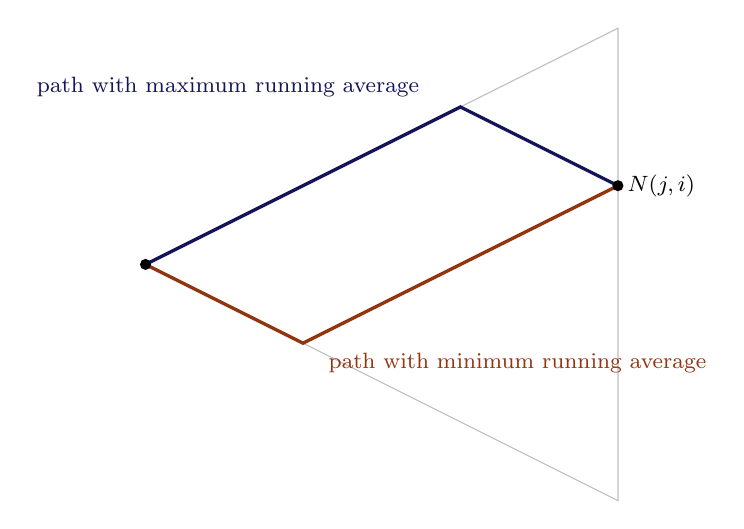
\begin{tikzpicture}[font=\footnotesize, x=1cm, y=0.5cm]
		\draw[Gray!50] (0,0) -- (6,6) -- (6,-6) -- cycle;
		\draw[MidnightBlue!80!black, very thick] (0,0) -- (4,4) -- (6,2);
		\draw[RawSienna, very thick] (0,0) -- (2,-2) -- (6,2);
		\fill (0,0) circle (2pt); \fill (6,2) circle (2pt) node[right] {$N(j,i)$};
		\node[MidnightBlue!80!black, anchor=south east] at (3.6,4) {path with maximum running average};
		\node[RawSienna, anchor=north west] at (2.2,-2) {path with minimum running average};
	\end{tikzpicture}
	\caption{All up moves first gives the largest running sum to $N(j,i)$, all
		down moves first the smallest; every other path lies in between.}
	\label{fig:max-min-paths}
\end{figure}

\zh{圖：先全部上漲得到最大的累積和，先全部下跌得到最小的；其他路徑都介於兩者之間。}

\source{Slides pp.~454--455}

The number of paths to $N(j,i)$ is far too large: $\binom{j}{i}$, and for example $\binom{j}{j/2}\sim2^{j}\sqrt{2/(\pi j)}$.
Moreover, the distribution of the running averages at any given time seems to be bimodal.\footnote{Contributed by Mr.~Liu, Jun (\texttt{R99944027}) on April 15, 2014. The slide's plot uses $n=24$, $u=5/4$ and $d=4/5$.}

\zh{到 $N(j,i)$ 的路徑數 $\binom{j}{i}$ 太多，例如 $\binom{j}{j/2}\sim2^{j}\sqrt{2/(\pi j)}$；而且某個時間點的 running average 分布似乎是雙峰的。}

\subsection{Bucketing}

\source{Slides pp.~456--458}

But all averages must lie between $A_{\min}(j,i)$ and $A_{\max}(j,i)$.
Pick $k+1$ equally spaced values in this range and treat them as the true and only running averages:
\[
	A_{m}(j,i) \;\triangleq\; \Bigl(\frac{k-m}{k}\Bigr)A_{\min}(j,i)+\Bigl(\frac{m}{k}\Bigr)A_{\max}(j,i) ,
	\qquad m=0,1,\ldots,k .
\]
Such \vocab{bucketing} or \vocab{binning} introduces errors, but it works reasonably well in practice.\footnote{J.~Hull \& White (1993); Ritchken, Sankarasubramanian, \& Vijh (1993).}
A better alternative picks values whose logarithms are equally spaced;\footnote{Called \vocab{log-linear interpolation}.} still other alternatives are possible, considering the bimodal distribution of averages.

\zh{所有平均都在 $A_{\min}$ 和 $A_{\max}$ 之間。在這範圍取 $k+1$ 個等距值，當成唯一可能的 running average。這種 bucketing（binning）有誤差，但實務上效果不錯。更好的做法是取對數等距的值；考慮到平均的分布是雙峰的，也可以有其他選法。}

\begin{remark}
	\vocab{分桶}（bucketing）：每個節點不再追蹤所有可能的平均值（指數多個），而是只保留 $A_{\min}$ 到 $A_{\max}$ 之間等距的 $k+1$ 個代表值，每個代表值各存一個選擇權價格。狀態數從指數降到 $O(kn^{2})$，代價是近似誤差。
	$A_{m}$ 的公式可以改寫成 $A_{m}=A_{\min}+m\cdot\frac{A_{\max}-A_{\min}}{k}$：從 $A_{\min}$ 開始，每格寬 $\frac{A_{\max}-A_{\min}}{k}$，$m=0$ 是 $A_{\min}$、$m=k$ 是 $A_{\max}$。
\end{remark}

\subsection{Backward Induction with Interpolation}

\source{Slides pp.~459--463}

Backward induction calculates the option values at each node for the $k+1$ running averages.
Suppose the current node is $N(j,i)$ and the running average is $a$, and consider the next node $N(j+1,i)$, after an up move.
As the asset price there is $S_{0}u^{j+1-i}d^{i}$, we seek the option value corresponding to the new running average
\[
	A_{u} \;\triangleq\; \frac{(j+1)\,a+S_{0}u^{j+1-i}d^{i}}{j+2} .
\]
But $A_{u}$ is not likely to be one of the $k+1$ running averages at $N(j+1,i)$!
Find the two running averages that bracket it,
\[
	A_{\ell}(j+1,i) \;\le\; A_{u} \;<\; A_{\ell+1}(j+1,i) .
\]
In ``most'' cases, the fastest way to nail $\ell$ is via
\[
	\ell \;=\; \left\lfloor\frac{A_{u}-A_{\min}(j+1,i)}{\bigl[A_{\max}(j+1,i)-A_{\min}(j+1,i)\bigr]/k}\right\rfloor .
\]
But watch out for
\begin{itemize}[nosep]
	\item the rare case where $A_{u}=A_{\ell}(j+1,i)$ for some $\ell$ (floating-point rounding may put it on either side);
	\item the case where $A_{u}=A_{\max}(j+1,i)$, which gives $\ell=k$ and no $A_{\ell+1}$;
	\item the degenerate case where $A_{0}(j+1,i)=\cdots=A_{k}(j+1,i)$, which happens to the two extreme paths ($i=0$ or $i=j+1$), where the formula divides by zero.
\end{itemize}

\zh{backward induction 要算每個 node 上 $k+1$ 個 running average 的 option 值。在 $N(j,i)$、running average 為 $a$ 時，上漲到 $N(j+1,i)$ 後新的 running average 是 $A_{u}$；它通常不是那裡的 $k+1$ 個值之一，所以找夾住它的 $A_{\ell}\le A_{u}<A_{\ell+1}$，$\ell$ 大多可用 floor 公式直接算。要注意三種情況：$A_{u}$ 剛好等於某個 $A_{\ell}$（浮點誤差可能讓它落到任一邊）；$A_{u}=A_{\max}$ 時 $\ell=k$、沒有 $A_{\ell+1}$；最邊緣的兩條路徑（$i=0$ 或 $i=j+1$）所有 $A_{\ell}$ 都相同，公式會除以零。}

\begin{remark}
	\begin{enumerate}[(1),nosep]
		\item \textbf{$A_{u}$。}running average $a$ 是 $S_{0},\ldots,S_{j}$ 共 $j+1$ 個價格的平均，所以總和是 $(j+1)a$；加上新價格 $S_{0}u^{j+1-i}d^{i}$ 後共 $j+2$ 個，再除以 $j+2$。
		\item \textbf{$\ell$。}由 bucketing 的改寫，$A_{\ell}=A_{\min}+\ell w$，$w=\frac{A_{\max}-A_{\min}}{k}$ 是格寬。$A_{\ell}\le A_{u}<A_{\ell+1}$ 等價於 $\ell\le\frac{A_{u}-A_{\min}}{w}<\ell+1$，所以取 floor。
		\item \textbf{三個例外。}(i) 浮點誤差可能讓 $A_{u}$ 剛好在格線上時算錯格；(ii) $A_{u}=A_{\max}$ 時 $\ell=k$，沒有第 $k+1$ 格；(iii) 最上、最下的 node 只有一條 path，$A_{\max}=A_{\min}$，$w=0$。
	\end{enumerate}
\end{remark}

\begin{figure}[H]
	\centering
	\begin{tikzpicture}[font=\footnotesize, every node/.style={inner sep=1pt}]
		\foreach \y/\l in {0.9/0, 0/m, -0.9/k} {\draw[thick] (0,\y) -- (0.6,\y); \node[left] at (-0.1,\y) {$\l$};}
		\node at (0.3,0.5) {$\vdots$}; \node at (0.3,-0.4) {$\vdots$};
		\foreach \s in {2.1,-2.1}{
				\begin{scope}[yshift=\s cm]
					\foreach \y in {1.0,0.3,-0.3,-1.0} \draw[thick] (3.6,\y) -- (4.2,\y);
					\node at (3.9,0.72) {$\vdots$}; \node at (3.9,-0.58) {$\vdots$};
					\node[right] at (4.3,1.0) {$0$}; \node[right] at (4.3,-1.0) {$k$};
				\end{scope}
			}
		\node[right] at (4.3,2.4) {$\ell$}; \node[right] at (4.3,1.8) {$\ell+1$};
		\node[right] at (4.3,-1.8) {$\ell'$}; \node[right] at (4.3,-2.4) {$\ell'+1$};
		\draw[-{Stealth[length=4pt]}, MidnightBlue!70!black] (3.55,2.1) -- (1.3,0) -- (0.65,0);
		\draw[MidnightBlue!70!black] (1.3,0) -- (3.55,-2.1);
		\node[font=\scriptsize, text=Gray!50!black, anchor=south east] at (2.3,1.1) {$N(j+1,i)$};
		\node[font=\scriptsize, text=Gray!50!black, anchor=north east] at (2.3,-1.1) {$N(j+1,i+1)$};
		\node[font=\scriptsize, text=Gray!50!black, anchor=south] at (0.3,1.15) {$N(j,i)$};
	\end{tikzpicture}
	\caption{Backward induction for arithmetic average-rate options. The $k+1$
		option values at $N(j,i)$ are stored in an array; each depends on two
		values at $N(j+1,i)$ (buckets $\ell$, $\ell+1$) and two at $N(j+1,i+1)$
		(buckets $\ell'$, $\ell'+1$).}
	\label{fig:asian-buckets}
\end{figure}

\zh{圖：$N(j,i)$ 的 $k+1$ 個 option 值存在一個 array；每個值取決於 $N(j+1,i)$ 的兩格（$\ell,\ell+1$）和 $N(j+1,i+1)$ 的兩格（$\ell',\ell'+1$）。}

Express $A_{u}$ as a linearly interpolated value of the two running averages,
\[
	A_{u} \;=\; x\,A_{\ell}(j+1,i)+(1-x)\,A_{\ell+1}(j+1,i) ,
	\qquad 0<x\le1 .
\]
Let $C_{\ell}(t,s)$ denote the option value at node $N(t,s)$ with running average $A_{\ell}(t,s)$.
Obtain the approximate option value given the running average $A_{u}$ via
\[
	C_{u} \;\triangleq\; x\,C_{\ell}(j+1,i)+(1-x)\,C_{\ell+1}(j+1,i) .
\]

\source{Slides pp.~464--466}

This interpolation introduces the second source of error; alternatives to linear interpolation exist.

\zh{把 $A_{u}$ 寫成兩格的線性內插 $xA_{\ell}+(1-x)A_{\ell+1}$，再用同樣的權重把兩格的 option 值內插成 $C_{u}$。這是第二個誤差來源；也有線性內插以外的做法。}

\begin{remark}
	\textbf{$x$ 怎麼算。}由 $A_{u}=xA_{\ell}+(1-x)A_{\ell+1}$ 解出 $x=\frac{A_{\ell+1}-A_{u}}{A_{\ell+1}-A_{\ell}}$。$A_{u}$ 越靠近 $A_{\ell}$，$x$ 越接近 $1$。$C_{u}$ 用同樣的權重 $x,1-x$ 把兩格的 option 價值加權，也就是假設 option 價值在兩格之間是 running average 的線性函數。
\end{remark}
The same steps are repeated for the down node $N(j+1,i+1)$ to obtain another approximate option value $C_{d}$.
Finally obtain the option value as
\[
	\bigl[\,pC_{u}+(1-p)\,C_{d}\,\bigr]e^{-r\Delta t} .
\]

\zh{對下跌的 node $N(j+1,i+1)$ 做同樣的事得到 $C_{d}$，最後 option 值是 $[pC_{u}+(1-p)C_{d}]e^{-r\Delta t}$。}

\begin{algorithm}[H]
	\caption{Approximation algorithm for European arithmetic average-rate calls}
	\label{alg:asian}
	\KwIn{$S_{0},u,d,X,n,\hat{r},k$}
	$p:=(e^{\hat{r}}-d)/(u-d)$\;
	\For(\tcp*[f]{terminal price $S_{0}u^{n-i}d^{i}$}){$i=0,1,\ldots,n$}{
		\For{$m=0,1,\ldots,k$}{$C[\,i\,][\,m\,]:=\max\bigl(0,\,A_{m}(n,i)-X\bigr)$\;}
	}
	\For{$j=n-1$ \KwTo $0$}{
		\For{$i=0,1,\ldots,j$}{
			\For{$m=0,1,\ldots,k$}{
				$a:=A_{m}(j,i)$\;
				$A_{u}:=\bigl((j+1)\,a+S_{0}u^{j+1-i}d^{i}\bigr)/(j+2)$\;
				find $\ell,x$ with $A_{u}=xA_{\ell}(j+1,i)+(1-x)A_{\ell+1}(j+1,i)$\;
				$C_{u}:=x\,C[\,i\,][\,\ell\,]+(1-x)\,C[\,i\,][\,\ell+1\,]$\;
				$A_{d}:=\bigl((j+1)\,a+S_{0}u^{j-i}d^{i+1}\bigr)/(j+2)$\;
				find $\ell',x'$ likewise at $N(j+1,i+1)$\;
				$C_{d}:=x'\,C[\,i+1\,][\,\ell'\,]+(1-x')\,C[\,i+1\,][\,\ell'+1\,]$\;
				$D[\,m\,]:=\bigl(pC_{u}+(1-p)\,C_{d}\bigr)e^{-\hat{r}}$\;
			}
			copy $D[\,0..k\,]$ to $C[\,i\,][\,0..k\,]$\;
		}
	}
	\Return{$C[\,0\,][\,0\,]$}\;
\end{algorithm}

\zh{完整演算法：先設好到期時每個 node、每個 bucket 的 payoff，再一欄一欄往回做上面的內插和 backward induction。}

\begin{note}
	需要先複製到 $D$，是因為下一個 $i$ 計算它的 $C_{d}$ 時還會讀 $C[\,i\,][\,\cdot\,]$ --- 和 \autoref{alg:bopm-european} 一樣是「proper updating」的問題。
	若是 American option，把對 $D[\,m\,]$ 的指定改成 $\max\bigl(a-X,\ (pC_{u}+(1-p)C_{d})e^{-\hat{r}}\bigr)$。
\end{note}

The running time is $O(kn^{2})$: there are $O(n^{2})$ nodes, and each node has $O(k)$ buckets.
No interpolation is needed for the calculations at time step $n-1$:\footnote{Contributed by Mr.~Chen, Shih-Hang (\texttt{R02723031}) on April 9, 2014.} the option values there are simply (for calls) $C_{u}=\max(A_{u}-X,0)$ and $C_{d}=\max(A_{d}-X,0)$, which saves $O(nk)$ calculations and one layer of error.

\zh{running time 是 $O(kn^{2})$：$O(n^{2})$ 個 node、每個 $O(k)$ 個 bucket。時間 $n-1$ 那一步不用內插：call 的值直接是 $C_{u}=\max(A_{u}-X,0)$、$C_{d}=\max(A_{d}-X,0)$，省下 $O(nk)$ 的計算和一層誤差。}

Arithmetic average-rate options were assumed to be newly issued, with no historical average to deal with.
This problem can be easily addressed:\footnote{See Exercise 11.7.4 of the textbook.} if the running sum of the first $m+1$ prices is $P$, the payoff is
\[
	\max\Bigl(\frac{P+\sum_{i=m+1}^{n}S_{i}}{n+1}-X,\ 0\Bigr)
	\;=\; \frac{n-m}{n+1}\,\max\Bigl(\frac{1}{n-m}\sum_{i=m+1}^{n}S_{i}-X',\ 0\Bigr) ,
\]
where $X'\triangleq\bigl[(n+1)X-P\bigr]/(n-m)$ ---
a scaled, newly issued option on the remaining prices with an adjusted strike (when $X'\le0$, the option is sure to finish in the money and is priced as a forward).

\zh{前面假設 option 是新發行的、沒有歷史平均。若前 $m+1$ 個價格的累積和是 $P$，payoff 可改寫成「只看剩下價格、strike 調整為 $X'$ 的新發行 option」再乘上 $\frac{n-m}{n+1}$（$X'\le0$ 時一定到價內，當作 forward 定價）。}

\begin{remark}
	\textbf{等式的驗證。}右邊括號內乘上 $\frac{n-m}{n+1}$：
	\[
		\frac{n-m}{n+1}\cdot\frac{1}{n-m}\sum_{i>m}S_{i}=\frac{\sum_{i>m}S_{i}}{n+1} ,
		\qquad
		\frac{n-m}{n+1}X'=\frac{(n+1)X-P}{n+1}=X-\frac{P}{n+1} ,
	\]兩者相減就是左邊括號內的 $\frac{P+\sum_{i>m}S_{i}}{n+1}-X$。再用 $c>0$ 時 $\max(cY,0)=c\max(Y,0)$。
\end{remark}
How about the Greeks?\footnote{Thanks to lively class discussions on March 31, 2004, and April 9, 2014.}
Delta and gamma from the first two periods (\autoref{sec:numerical-greeks}) are available as before, but each $f_{u}$ and $f_{d}$ now carries bucketing and interpolation errors of its own, which the difference quotients amplify.

\zh{Greeks 呢？前兩期的 delta、gamma 照樣可用（\autoref{sec:numerical-greeks}），但每個 $f_{u}$、$f_{d}$ 都帶有 bucketing 和內插誤差，差商會把誤差放大。}

\subsection{A Numerical Example}
\label{sec:asian-example}

\source{Slides pp.~467--473}

Consider a European arithmetic average-rate call with strike price $50$, and assume zero interest rate in order to dispense with discounting.
The tree has $u=1.069$, $d=0.936$, $p=0.483$ and $S_{0}=50$.
Node A is 2 periods from the root (price $50$, after one up and one down move); its successors B and C are at expiration, with prices $53.447$ and $46.775$.
Each node picks $k=3$, i.e., 4 equally spaced running averages (\autoref{fig:asian-example}).
The minimum running average at node A is $48.925$, the maximum $51.149$.

\zh{例子：strike 50 的 European 算術 average-rate call，利率設為 $0$ 免折現；$u=1.069$、$d=0.936$、$p=0.483$、$S_{0}=50$。node A 在兩期後（一漲一跌，股價 50），後繼 B、C 在到期，股價 53.447、46.775。每個 node 取 $k=3$（4 個等距 running average）；A 的最小、最大 running average 是 48.925、51.149。}

\begin{remark}
	\begin{enumerate}[(1),nosep]
		\item \textbf{A 的 $A_{\min},A_{\max}$。}A 是一漲一跌，到 A 的兩條 path 中先跌的平均最小：$\frac{S_{0}+S_{0}d+S_{0}du}{3}$；先漲的最大：$\frac{S_{0}+S_{0}u+S_{0}ud}{3}$。
		\item \textbf{四個 bucket。}格寬 $\frac{51.149-48.925}{3}$，所以四個值是 $48.925$、$49.666$、$50.408$、$51.149$（\autoref{fig:asian-example}）。
		\item \textbf{B、C 的 option 值。}B、C 在到期，option 值就是 payoff $\max(\text{average}-50,0)$。
	\end{enumerate}
\end{remark}

\begin{figure}[H]
	\centering
	\begin{tikzpicture}[font=\scriptsize, every node/.style={inner sep=1.5pt}]
		\node (A) at (0,0) {
			\begin{tabular}{|c|c|}\hline
				48.925 & 0.0269 \\ \hline
				49.666 & 0.2956 \\ \hline
				50.408 & 0.5782 \\ \hline
				51.149 & 0.8617 \\ \hline
			\end{tabular}};
		\node[above=1pt of A] {$50$};
		\node[below=1pt of A] {A};
		\node (B) at (5.2,2.0) {
			\begin{tabular}{|c|c|}\hline
				50.056 & 0.056 \\ \hline
				51.206 & 1.206 \\ \hline
				52.356 & 2.356 \\ \hline
				53.506 & 3.506 \\ \hline
			\end{tabular}};
		\node[above=1pt of B] {$53.447$};
		\node[below=1pt of B] {B};
		\node (C) at (5.2,-2.0) {
			\begin{tabular}{|c|c|}\hline
				46.827 & 0.000 \\ \hline
				47.903 & 0.000 \\ \hline
				48.979 & 0.000 \\ \hline
				50.056 & 0.056 \\ \hline
			\end{tabular}};
		\node[above=1pt of C] {$46.775$};
		\node[below=1pt of C] {C};
		\draw[MidnightBlue!70!black] (A.east) -- node[above, sloped] {$50.612$} (B.west);
		\draw[MidnightBlue!70!black] (A.east) -- node[below, sloped] {$48.944$} (C.west);
		\node[draw, align=left, font=\scriptsize] at (1.0,-2.6) {$u=1.069$\\$d=0.936$\\$p=0.483$};
	\end{tikzpicture}
	\caption{Running averages (left columns) and option values at node A and its two
		successors. The edges show the new averages reached from A's second bucket,
		$49.666$.}
	\label{fig:asian-example}
\end{figure}

\zh{圖：node A 和兩個後繼的 running average（左欄）與 option 值；連線是從 A 的第二格 49.666 出發到達的新平均。}

Consider the up move from node A with running average $49.666$.
Because the stock price at node B is $53.447$, the new running average is
\[
	\frac{3\times49.666+53.447}{4} \;\approx\; 50.612 .
\]
With $50.612$ lying between $50.056$ and $51.206$ at node B, we solve $50.612=x\times50.056+(1-x)\times51.206$ to obtain $x\approx0.517$.
The option values corresponding to running averages $50.056$ and $51.206$ at node B are $0.056$ and $1.206$, so their contribution is weighted linearly as
\[
	x\times0.056+(1-x)\times1.206 \;\approx\; 0.611 .
\]

Now consider the down move.
Because the stock price at node C is $46.775$, the new running average is $(3\times49.666+46.775)/4\approx48.944$, lying between $47.903$ and $48.979$, so $x\approx0.033$.
The option values there are both $0.0$, so the contribution is $0.0$.
Finally, the option value corresponding to running average $49.666$ at node A equals
\[
	p\times0.611+(1-p)\times0.0 \;\approx\; 0.2956 ,
\]
where $p=0.483$.
The remaining three option values at node A can be computed similarly.

\zh{從 A 的 49.666 往上：B 的新平均 $(3\times49.666+53.447)/4\approx50.612$，介於 50.056 和 51.206，$x\approx0.517$，內插得 $0.611$。往下：C 的新平均 48.944，介於 47.903 和 48.979，兩格的值都是 $0$。所以 A 這一格的值是 $0.483\times0.611\approx0.2956$；其他三格同理。}

\begin{remark}
	\begin{enumerate}[(1),nosep]
		\item \textbf{$x$。}$x=\frac{51.206-50.612}{51.206-50.056}\approx0.517$，套上面 interpolation 的公式。
		\item \textbf{沒有折現。}利率為 $0$，所以 backward induction 只是 $pC_{u}+(1-p)C_{d}$，不用乘 $e^{-r\Delta t}$。
	\end{enumerate}
\end{remark}

\begin{note}
	A 在時間 $n-1$，所以由上面的 shortcut 不需要 interpolation：精確計算 $C_{u}=\max(50.612-50,0)=0.612$，價值為 $0.2955$ --- 在這裡幾乎一樣。
	第三個 bucket（$50.408$）差得比較多：interpolation 給出 $0.578$，精確計算是 $0.564$。
	原因是 option 價值對 running average 是 \emph{convex} 的（到期時是 $\max(\cdot-X,0)$），所以 linear interpolation 用的弦會落在函數上方。
	這正是下一個 remark 背後的機制。
\end{note}

%─────§ Remarks──────────────────────────────────────────────────────────────────────────────────────────────────────────────────────────────────────
\subsection{Remarks on Asian Option Pricing}

\source{Slides pp.~474--478}

Asian option pricing is an active research area.
\begin{itemize}[itemsep=0.3em]
	\item The above algorithm overestimates the ``true'' value, and to guarantee convergence, $k$ needs to grow with $n$ at least.\footnote{T.~Dai (\texttt{B82506025}, \texttt{R86526008}, \texttt{D8852600}), G.~Huang (\texttt{F83506075}), \& Lyuu (2002). With $k=50000$ the slide's plot of the value against $n=50,\ldots,140$ still drifts between about $0.325$ and $0.35$.}
	\item There is a convergent approximation algorithm that does away with interpolation, with a running time of $2^{O(\sqrt{n})}$.\footnote{T.~Dai (\texttt{B82506025}, \texttt{R86526008}, \texttt{D8852600}) \& Lyuu (2002, 2004).}
	\item There is an $O(kn^{2})$-time algorithm with an error bound of $O(Xn/k)$ from the naive $O(2^{n})$-time binomial tree algorithm in the case of European Asian options.\footnote{Aingworth, Motwani (1962--2009), \& Oldham (2000).}
	      $k$ can be varied for trade-off between time and accuracy: picking $k=O(n^{2})$ gives an error of $O(1/n)$ and a running time of $O(n^{4})$.
	\item Another approximation algorithm reduces the error to $O(X\sqrt{n}/k)$ by varying the number of buckets per node.\footnote{T.~Dai (\texttt{B82506025}, \texttt{R86526008}, \texttt{D8852600}), G.~Huang (\texttt{F83506075}), \& Lyuu (2002).}
	      If we pick $k=O(n)$, the error is $O(n^{-0.5})$; if we pick $k=O(n^{1.5})$, the error is $O(1/n)$ and the running time is $O(n^{3.5})$.
	\item Under ``reasonable assumptions,'' an $O(n^{2})$-time algorithm with an error bound of $O(1/n)$ exists.\footnote{Hsu (\texttt{R7526001}, \texttt{D89922012}) \& Lyuu (2004).}
	      The basic idea is a nonuniform allocation of running averages $k_{ij}$ instead of a uniform $k$: few buckets where the range $A_{\max}-A_{\min}$ is narrow (near the edges of the tree), many where it is wide.
	      It strikes a tight balance between error and complexity.
\end{itemize}

\zh{Asian option 定價是活躍的研究領域：上面的演算法會高估真值，要保證收斂 $k$ 至少要隨 $n$ 成長；有不需內插、$2^{O(\sqrt{n})}$ 時間的收斂近似演算法；有 $O(kn^{2})$ 時間、誤差 $O(Xn/k)$ 的演算法，取 $k=O(n^{2})$ 得 $O(1/n)$ 誤差、$O(n^{4})$ 時間；讓每個 node 的 bucket 數不同可把誤差降到 $O(X\sqrt{n}/k)$；在合理假設下有 $O(n^{2})$ 時間、$O(1/n)$ 誤差的演算法，關鍵是 bucket 數 $k_{ij}$ 不均勻：$A_{\max}-A_{\min}$ 窄處（tree 邊緣）少放、寬處多放。}

\begin{intuition}
	Why can a nonuniform allocation help so much?
	The bucketing error at a node is proportional to the bucket width $(A_{\max}-A_{\min})/k$.
	That range is zero on the two edges of the tree and widest in the middle, so spending the same $k$ everywhere wastes buckets where they are not needed.
\end{intuition}

\zh{為什麼不均勻分配幫助這麼大？每個 node 的 bucketing 誤差和格寬 $(A_{\max}-A_{\min})/k$ 成正比；這個範圍在 tree 兩側邊緣是 $0$、中間最寬，所以每處都放同樣的 $k$ 會把 bucket 浪費在不需要的地方。}

\subsection{A Grand Comparison}

\source{Slides pp.~479--481}

The slides compare several methods against exact values over a grid of strikes, volatilities and rates.\footnote{Hsu (\texttt{R7526001}, \texttt{D89922012}) \& Lyuu (2004); J.~E.~Zhang (2001, 2003); K.~Chen (\texttt{R92723061}) \& Lyuu (2006).}
AA2 and AA3 are Zhang's analytical approximations; Hsu--Lyuu is the $O(n^{2})$ tree; Chen--Lyuu is the formula above.
A selection:

\begin{table}[H]
	\centering
	\small
	\begin{tabular}{rrrrrrrr}
		\toprule
		$X$ & $\sigma$ & $r$  & Exact      & AA2        & AA3        & Hsu--Lyuu & Chen--Lyuu \\
		\midrule
		95  & 0.05     & 0.05 & 7.1777275  & 7.1777244  & 7.1777279  & 7.178812  & 7.177726   \\
		100 &          &      & 2.7161745  & 2.7161755  & 2.7161744  & 2.715613  & 2.716168   \\
		105 &          &      & 0.3372614  & 0.3372601  & 0.3372614  & 0.338863  & 0.337231   \\
		\midrule
		90  & 0.10     & 0.05 & 11.9510927 & 11.9509331 & 11.9510871 & 11.951610 & 11.951076  \\
		100 &          &      & 3.6413864  & 3.6414032  & 3.6413875  & 3.642325  & 3.641344   \\
		110 &          &      & 0.3312030  & 0.3312563  & 0.3311968  & 0.331348  & 0.331074   \\
		\midrule
		90  & 0.30     & 0.05 & 13.9538233 & 13.9555691 & 13.9540973 & 13.953937 & 13.952421  \\
		100 &          &      & 7.9456288  & 7.9459286  & 7.9458549  & 7.945918  & 7.944357   \\
		110 &          &      & 4.0717942  & 4.0702869  & 4.0720881  & 4.071945  & 4.070115   \\
		\midrule
		90  & 0.30     & 0.15 & 16.5129113 & 16.5133090 & 16.5128376 & 16.512963 & 16.512024  \\
		100 &          &      & 10.2098305 & 10.2110681 & 10.2101058 & 10.210039 & 10.208724  \\
		110 &          &      & 5.7301225  & 5.7296982  & 5.7303567  & 5.730357  & 5.728161   \\
		\bottomrule
	\end{tabular}
	\caption{Arithmetic average-rate call values from the slides' comparison
		(rows for $\sigma=0.05,0.10,0.30$; the slides also cover $\sigma=0.20$ and
		$r=0.09,0.15$ throughout).}
	\label{tab:asian-comparison}
\end{table}

\zh{簡報在一組 strike、波動率、利率上比較幾種方法和精確值：AA2、AA3 是 Zhang 的解析近似，Hsu--Lyuu 是 $O(n^{2})$ 的 tree，Chen--Lyuu 是上面的近似公式。表中是部分結果。}

\begin{moral}
	All four methods agree to about three or four significant digits across the board; the analytical approximations lose digits as $\sigma$ grows, the tree is weakest at small $\sigma$.
	A problem whose naive solution is exponential is, in practice, solved --- but every method trades accuracy, time and guarantees differently, and only some of them come with error bounds.
\end{moral}

\zh{四種方法大致都準到三、四位有效數字；解析近似在 $\sigma$ 大時失準，tree 在 $\sigma$ 小時最弱。天真解法是指數時間的問題，實務上已經解決——但每種方法在準確度、時間和保證之間的取捨不同，只有部分方法有誤差上界。}
